\documentclass[12pt, oneside]{article}
\usepackage{pdfpages}
\usepackage[english]{babel}
\usepackage[numbers]{natbib}
\usepackage{url}
\usepackage[utf8x]{inputenc}
\usepackage{amsmath}
\usepackage{graphicx}
\graphicspath{{images/}}
\usepackage{parskip}
\usepackage{fancyhdr}
\usepackage{textcomp}
\usepackage{fancyhdr}
\setlength{\footskip}{14.5pt}
\usepackage{array}
\usepackage{setspace}
\usepackage{hyperref}
\usepackage{float}
\usepackage{longtable}
\usepackage{caption}
\usepackage{hyperref}
\usepackage[numbers]{natbib}
\usepackage[a4paper, top=2.5cm, bottom=1.25cm, inner=3.5cm, outer=1.25cm]{geometry}
\usepackage{sectsty}
\sectionfont{\fontsize{16pt}{16pt}\selectfont}
\subsectionfont{\fontsize{14pt}{14pt}\selectfont}
\hypersetup{
colorlinks=true,
    linkcolor=blue,
    filecolor=magenta,      
    urlcolor=blue,
    citecolor=blue
}


\pagestyle{fancy}
\fancyhf{}                      % Clear default header/footer
\renewcommand{\headrulewidth}{0pt}  % Remove top line
\renewcommand{\footrulewidth}{0pt}  % Remove bottom line

\fancyfoot[C]{\thepage}         % Centered page number in footer

\setlength{\footskip}{10pt}     % Adjust this value upward if too low

\title{\textit{Guru Nanak Dev Engineering College, Ludhiana}	}				
% \author{\textit{Brahamjot Singh}}



% \pagestyle{fancy}
% \fancyhf{}
% \rhead{\theauthor}
% \lhead{\thetitle}
% \cfoot{\thepage}

\begin{document}
    
\begin{titlepage}
\begin{center}
	\centering
    % \vspace*{0.25 cm}\textbf{\fontsize{14pt}{14pt}\selectfont Major Project Report}\\[0.5 cm]
     % \textbf{\fontsize{14pt}{14pt}\selectfont on}\\[0.5 cm]
     \textbf{\fontsize{24pt}{24pt}\selectfont Trackit}\\[1.5 cm]
     \textbf{\fontsize{14pt}{14pt}\selectfont REPORT}\\[0.5 cm]
     {\fontsize{12pt}{12pt}\selectfont SUBMITTED IN PARTIAL FULFILLMENT OF THE REQUIREMENT FOR\\ Six Months Industrial Training (TR-104)}\\[0.5 cm]
     \textbf{\fontsize{14pt}{14pt}\selectfont at}\\[0.5 cm]
    \vspace*{0.25 cm}\textbf{\fontsize{14pt}{14pt}\selectfont AURIBISES TECHNOLOGIES PVT. LTD.}\\[0.25 cm]
    \vspace*{0.25 cm}\textbf{\fontsize{14pt}{14pt}\selectfont (from \underline{January} to \underline{May} 2026)}\\[1 cm]
    {\fontsize{14pt}{14pt}\selectfont{\textbf{Submitted by:}}\\[0.25cm]
    Aarchie Maggu (URN: 2203784)\\[0.25cm]
    Arshdeep Kaur (URN: 2203804)\\[0.25cm]
    Brahamjot Singh (URN: 2303081)}\\[1.25cm]
    
\includegraphics[scale = 0.17]{logo.png}\\[2cm]	
	\begin{center}
    \textbf{\fontsize{14pt}{14pt}\selectfont Department of Information Technology}\\
\end{center}
 	\begin{center}
    \textbf{\fontsize{14pt}{14pt}\selectfont Guru Nanak Dev Engineering College}\\
\end{center}
\begin{center}
    \textbf{\fontsize{14pt}{14pt}\selectfont Ludhiana, INDIA}\\
\end{center}
	\vfill
\end{center}
\end{titlepage}

\doublespacing
\pagenumbering{roman}
\newpage
\begin{center}
    \section*{CERTIFICATE BY THE COMPANY}
    \addcontentsline{toc}{section}{CERTIFICATE BY THE COMPANY}
    
    \vspace{1em}
    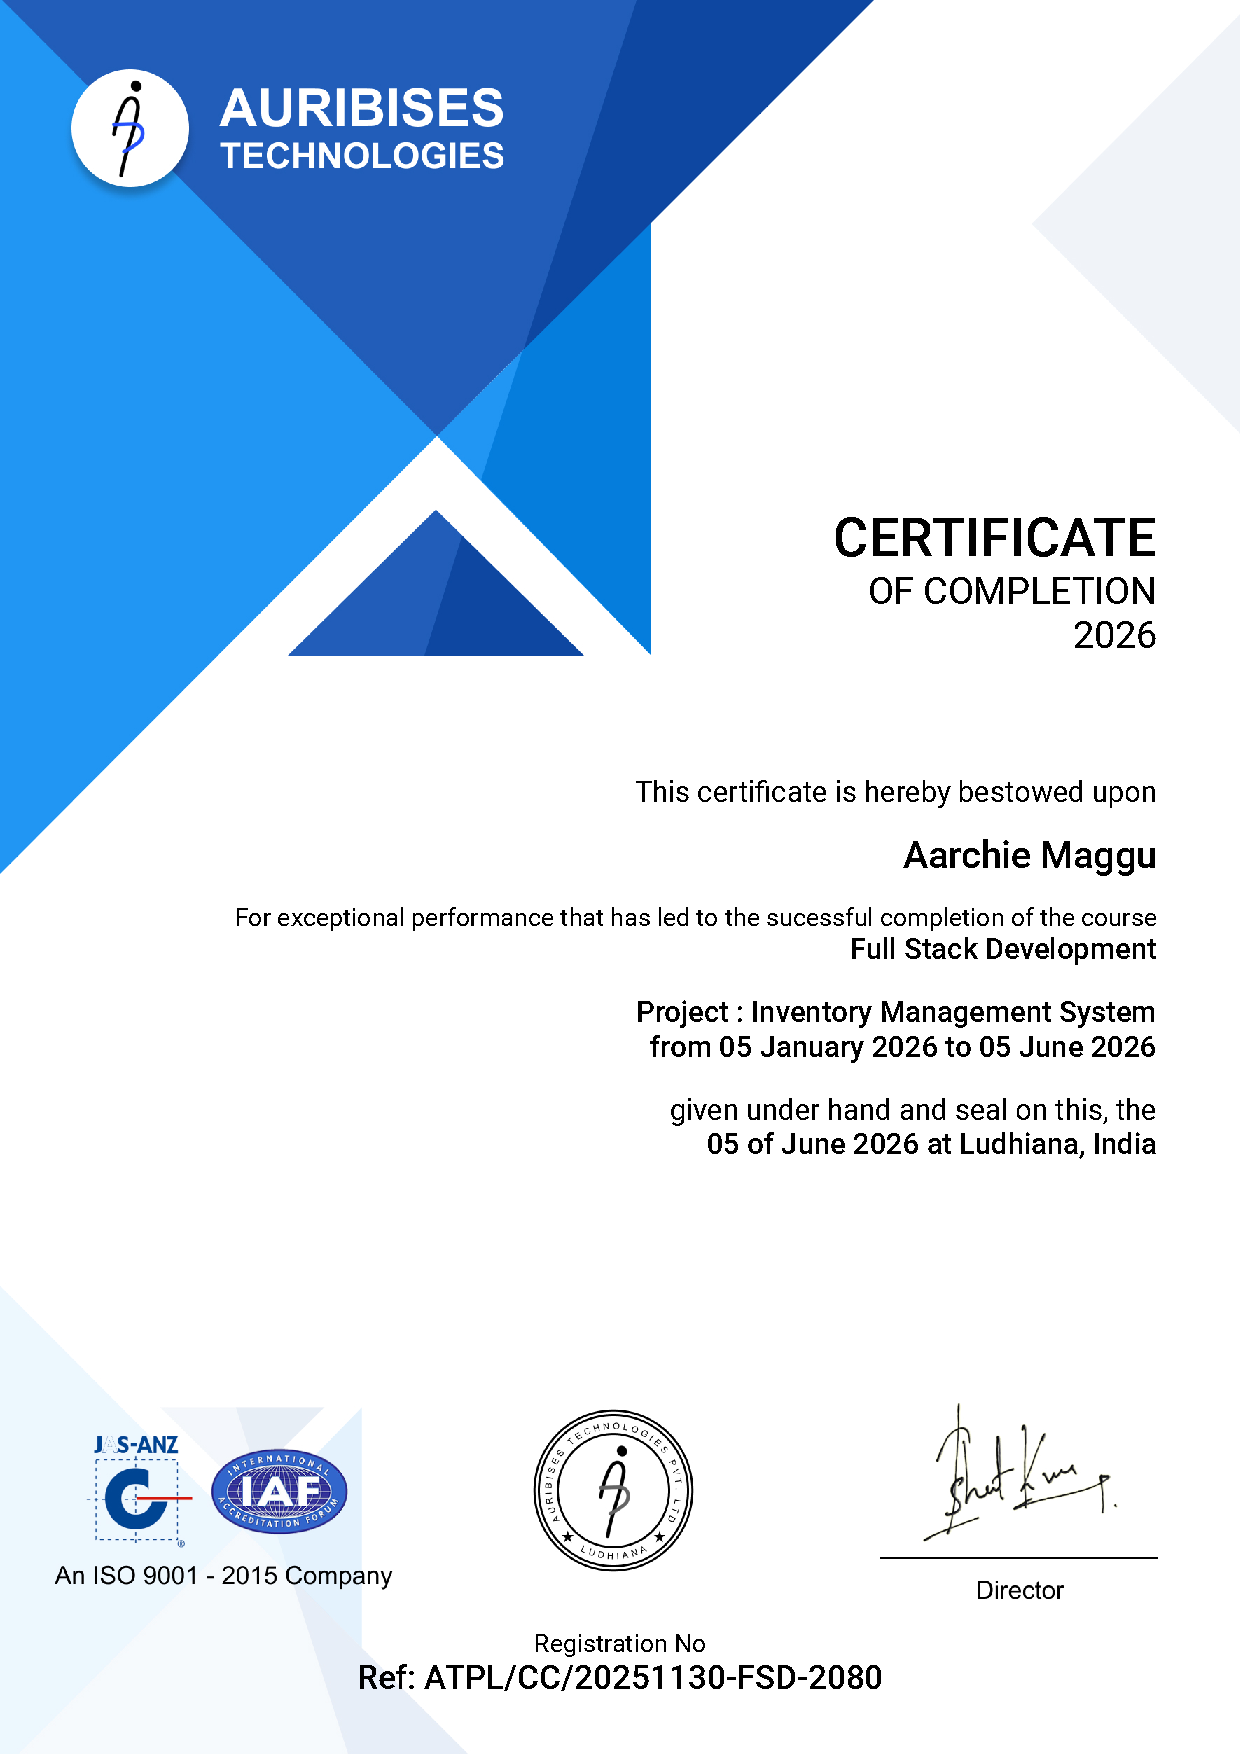
\includegraphics[page=1,width=\linewidth]{certificates/Aarchie.pdf}
\end{center}
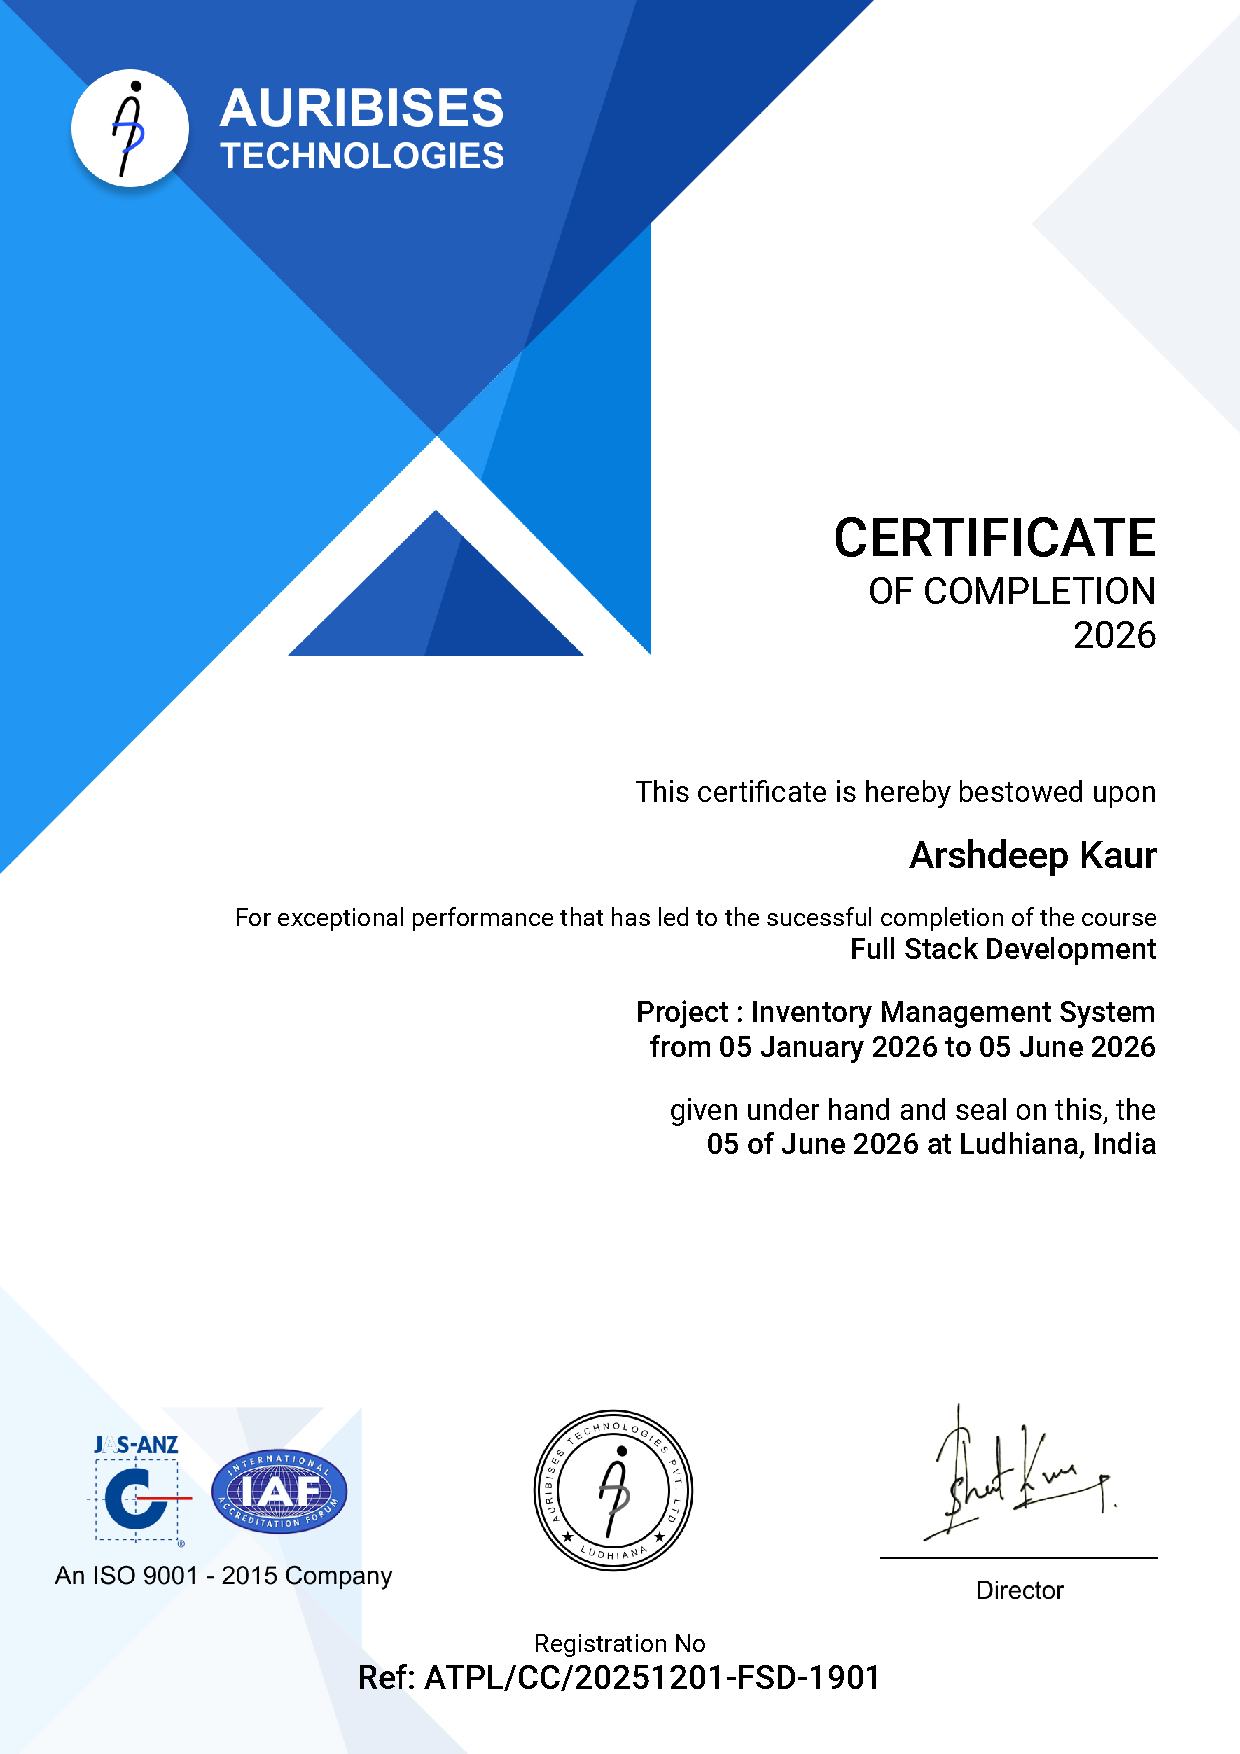
\includepdf[pages=1]{certificates/Arshdeep.pdf}
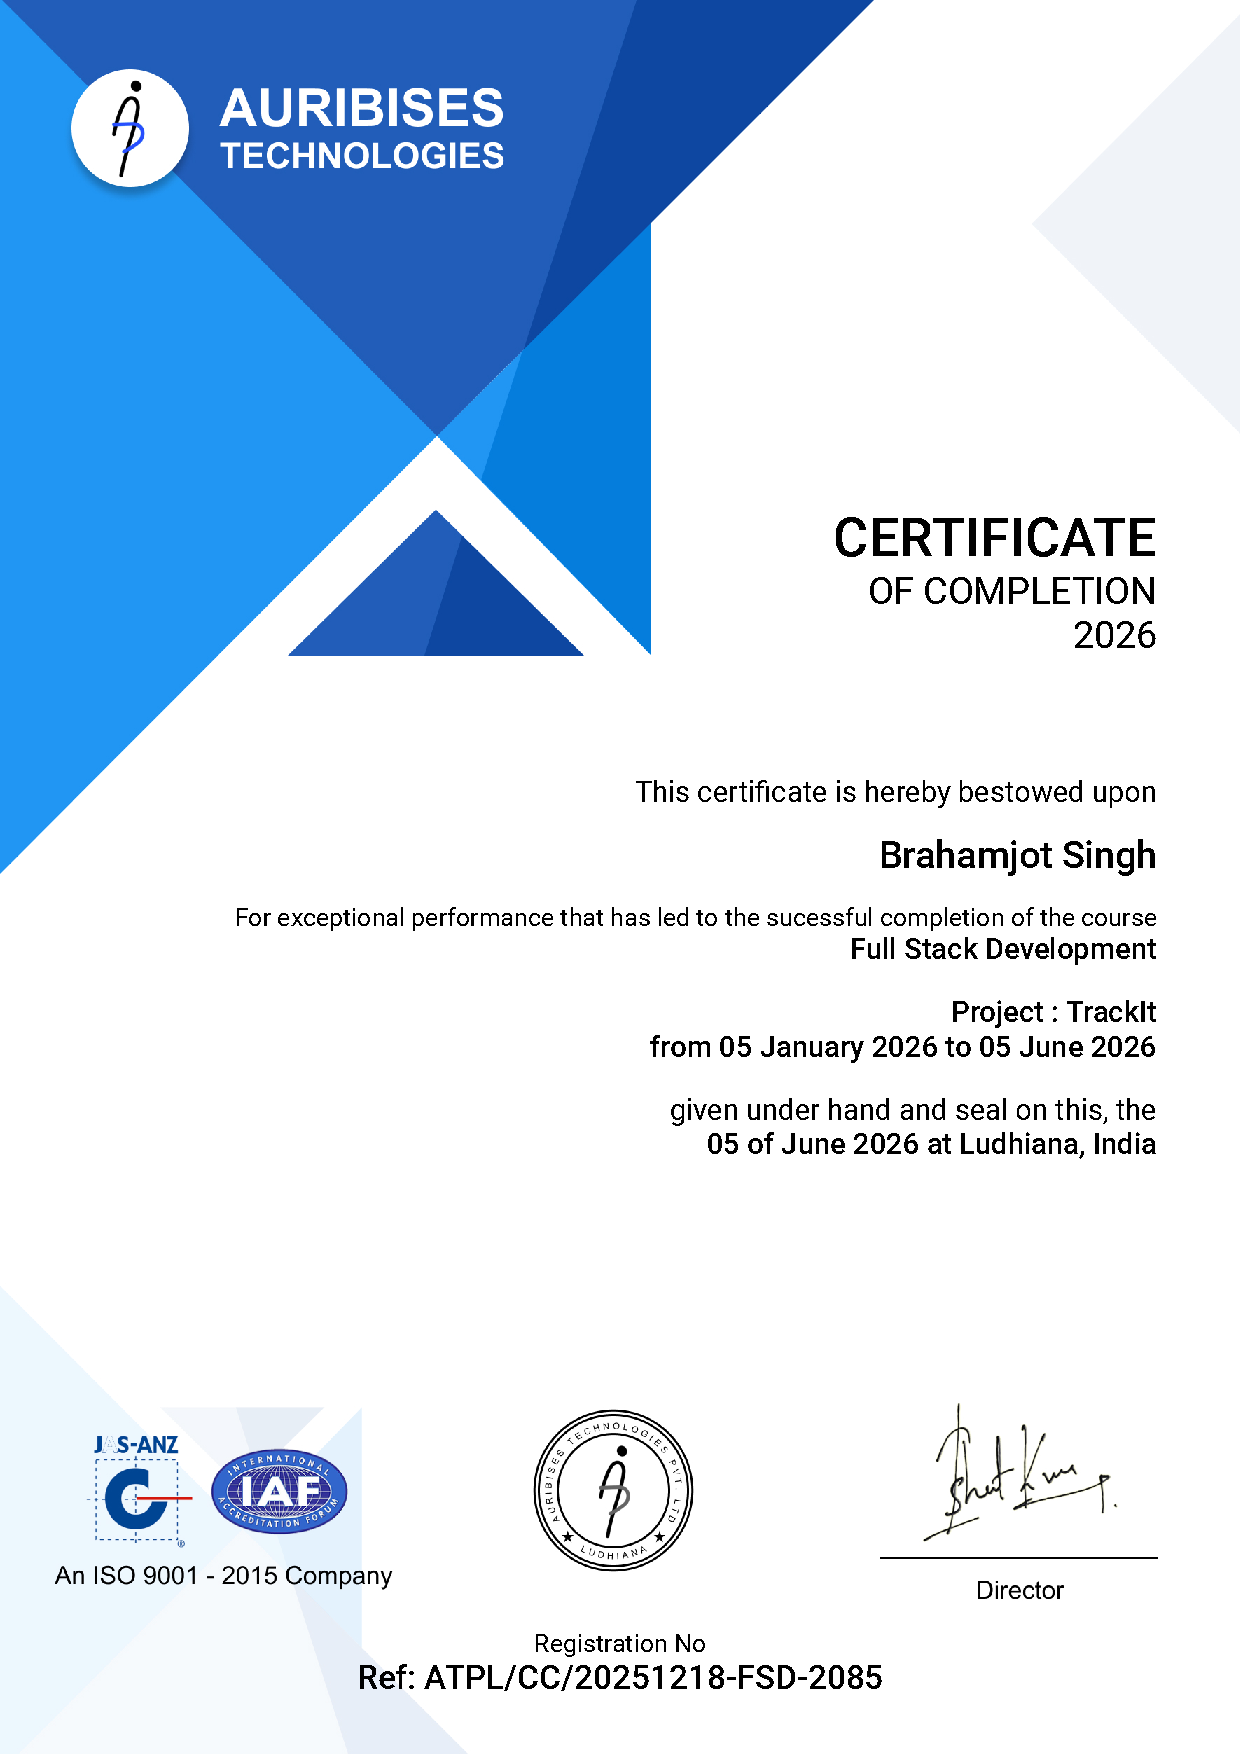
\includepdf[pages=1]{certificates/Brahamjot.pdf}

\newpage
\begin{center}
    \section*{CANDIDATE'S DECLARATION}
    \addcontentsline{toc}{section}{CANDIDATE'S DECLARATION}
\end{center}
\doublespacing
We hereby declare that I have undertaken Six month training at “Auribises Technologies Pvt. Ltd.” during a period from \underline{January 2026} to \underline{June 2026} in partial fulfillment of requirements for the award of degree of B.Tech (Information Technology) at GURU NANAK DEV ENGINEERING COLLEGE, LUDHIANA. The work which is being presented in the training report submitted to Department of Information Technology at GURU NANAK DEV ENGINEERING COLLEGE, LUDHIANA is an authentic record of training work.\\[3.5cm]
\textbf{Signature of the Students}\\[2.5cm]
The six month industrial training Viva–Voce Examination of \rule{3cm}{0.4pt} has been held on \rule{3cm}{0.4pt} and accepted.\\[3.5cm]
\begin{minipage}{0.45\textwidth}
    \begin{flushleft}
        \textbf{Signature of Internal Examiner}
    \end{flushleft}
\end{minipage}
\hfill % Pushes the next minipage to the absolute right margin
\begin{minipage}{0.45\textwidth}
    \begin{flushright}
        \textbf{Signature of External Examiner}
    \end{flushright}
\end{minipage}


\newpage
\begin{center}
    \section*{ABSTRACT}
    \addcontentsline{toc}{section}{ABSTRACT}
\end{center}
\doublespacing
Trackit is a SaaS-based Inventory Management System developed specifically for tyre dealers to simplify and centralize the process of managing customer records, inventory, and sales data. Traditionally, many dealers maintain customer and sales records manually through applications such as WhatsApp or physical registers, which leads to inefficiency, data redundancy, and difficulty in tracking customer history. The objective of this project is to reduce manual effort and provide a structured digital platform for managing business operations efficiently.\\[0.25cm]
The system consists of a NextJS {nextjs}-based web portal and a Flutter \cite{flutter}-based cross-\citeplatform mobile application integrated through Firebase \cite{firebase} services. The web portal allows dealers to securely log in, create worker accounts, manage permissions, and monitor overall shop inventory and operations. The mobile application enables both dealers and workers to access features based on assigned permissions. Key functionalities include customer management, daybook maintenance, sales tracking, inventory management using room and stack organization, report generation, and daily sales monitoring. The application also includes features such as dark mode support and a cart-based sales logging system for improved usability.\\[0.25cm]
The project utilizes Flutter for mobile application development, NextJS for the web portal, Firebase for authentication, database management, hosting, and real-time synchronization, while Vercel \cite{vercel} is used for deploying the web application. Trackit provides an efficient, scalable, and user-friendly solution for tyre dealers to digitally manage their business operations and customer records from a centralized platform.


\newpage
\begin{center}
    \section*{ACKNOWLEDGMENT}
    \addcontentsline{toc}{section}{ACKNOWLEDGMENT}
\end{center}
We are highly grateful to the Dr. Sehijpal Singh , Principal, Guru Nanak Dev Engineering College (GNDEC), Ludhiana, for providing this opportunity to carry out Six Months industrial training at \underline{Auribises Technologies Pvt. Ltd.}\\[0.25cm]
The constant guidance and encouragement received from Dr. K. S. Mann, Head of the Department, GNDEC Ludhiana has been of great help during the training and project work and is acknowledged with reverential thanks.\\[0.25cm]
We would like to express a deep sense of gratitude and thanks profusely to Ishant Kumar, CEO, Auribises Technologies. Pvt. Ltd. Without his wise counsel and able guidance, it would have been impossible to complete the report in this manner.\\[0.25cm]
We express gratitude to other faculty members of Information Technology department of GNDEC for their intellectual support throughout the course of this work.\\[0.25cm]
Finally, We are indebted to all whosoever have contributed in this report work and friendly stay at Auribises Technologies Pvt. Ltd.\\[0.5cm]

\textbf{Aarchie Maggu}\\[0.5cm]
\textbf{Arshdeep Kaur}\\[0.5cm]
\textbf{Brahamjot Singh}\\[0.5cm]

\newpage
\begin{center}
    \section*{ABOUT THE COMPANY}
    \addcontentsline{toc}{section}{ABOUT THE COMPANY}
\end{center}

Auribises Technologies Pvt. Ltd. is a software development and technology consulting company established in November 2011. The company specializes in mobile application development, web application development, cloud-based solutions, Artificial Intelligence (AI), and enterprise software systems. Auribises provides end-to-end software engineering services that help organizations streamline operations, improve productivity, and achieve their business objectives through technology-driven solutions. The company website, https://auribises.com \cite{auribises}, serves as a platform to showcase its services, products, training programs, and technological innovations.
\\[0.25cm]
At Auribises, we just not only develop, but also provide educational services that helps students to hone their technical skills. Auribises offers a unique combination of technical competencies with practical exposure on ongoing projects to its students. Auribises has a core vision for lightening thousands of candles with a single candle and hence we believe that it is our endeavor to continually share our learning’s with the larger world.\\[0.25cm]
Our objective is to surpass customer expectations consistently. Auribises Technologies delivers Software Engineering Services and technology-driven Business Solutions that help meet the business objectives of our clients. We work constantly towards creating values in business for our customers, employees and partners. Auribises aims to maximize talent by empowering individuals and organizations for development.

\newpage
\begin{center}
    \section*{LIST OF FIGURES}
    \addcontentsline{toc}{section}{LIST OF FIGURES}
\end{center}
\listoffigures

\newpage
\begin{center}
    \section*{LIST OF TABLES}
    \addcontentsline{toc}{section}{LIST OF TABLES}
\end{center}
\listoftables


\newpage
\begin{center}
    \section*{INDEX}
    \addcontentsline{toc}{section}{INDEX}
\end{center}
\tableofcontents



\newpage
\pagenumbering{arabic} % Switch to Arabic numbers
\setcounter{page}{1}

\begin{center}
    \section*{Chapter 1: Introduction}
    \addcontentsline{toc}{section}{1. Introduction}
\end{center}

\subsection*{1.1 Introduction to Organization}
\addcontentsline{toc}{subsection}{1.1 Introduction to Organization}
\textbf{Auribises Technologies} delivers Software Engineering Services and technology-driven Business Solutions that help meet the business objectives of clients. Founded in November 2011, Auribises has established unparalleled domain competencies in mobile and web technologies. The company specializes in developing cloud-based mobile applications, web applications, and innovative solutions powered by Artificial Intelligence.\\[0.25cm]
Auribises focuses on powering the connected age by designing and developing native mobile applications for both Android and iOS platforms. The company offers a complete suite of mobile, web, and software applications tailored to industry needs. With a strong foundation in modern technologies and scalable development practices, Auribises continues to take on critical challenges faced by the industry.\\[0.25cm]
The organization operates on a strong values-based culture that emphasizes integrity, transparency, and corporate governance. The core value system of Auribises is driven by the three D's: \textbf{DIVE}, \textbf{DEVELOP}, and \textbf{DELIVER}. These principles guide the company in maintaining the highest ethical standards while consistently delivering quality solutions to clients and partners.\\[0.25cm]
Auribises is committed to providing expert software engineering services using cutting-edge technologies and industry best practices. The company offers full-stack solutions, ranging from mobile and web application development to cloud infrastructure and AI-driven innovations. By leveraging modern technologies and artificial intelligence, Auribises helps businesses stay ahead in a rapidly evolving digital landscape.\\[0.25cm]
Apart from software development, Auribises also contributes significantly to technical education and skill development. The company provides educational services that help students enhance their technical capabilities through practical exposure to real-world projects. Auribises believes in sharing knowledge and empowering learners, following its vision of “lightening thousands of candles with a single candle.”\\[0.25cm]
Customer satisfaction remains a primary objective at Auribises. The company continuously works towards exceeding customer expectations while creating value for clients, employees, and business partners. Through reliable partnerships, scalable solutions, and dedicated support, Auribises aims to maximize talent by empowering individuals and organizations for growth and development.\\[0.25cm]
\textbf{Why Choose Auribises}
\begin{itemize}
    \item \textbf{Expert Development:} Professional software engineering with cutting-edge technologies and best practices.
    
    \item \textbf{Full-Stack Solutions:} End-to-end development from mobile applications to web platforms and cloud infrastructure.
    
    \item \textbf{AI \& Innovation:} Advanced solutions powered by Artificial Intelligence and modern technologies.
    
    \item \textbf{Trusted Partnership:} Reliable, scalable solutions with dedicated support focused on client success.
\end{itemize}

\subsection*{1.2 Introduction to Project}
\addcontentsline{toc}{subsection}{1.2 Introduction to Project}
Trackit is a SaaS \cite{saas}-based Inventory Management System designed specifically for tyre dealers, wholesalers, and retailers to simplify the process of managing customer records, inventory, sales, and employee operations through a centralized digital platform. The project aims to replace traditional methods of record keeping such as registers, notebooks, and messaging applications like WhatsApp, which often become difficult to manage as the customer database grows over time.\\[0.25 cm]
In the tyre business, maintaining accurate customer and sales records is extremely important for tracking tyre purchases, warranty claims, vehicle running history, and future customer servicing. Large dealers often face challenges in identifying which customer purchased a specific tyre, on what date it was purchased, and how much distance the vehicle has travelled since the installation of new tyres or any other service the dealer provides. Manual record management consumes significant time, increases the possibility of errors, and makes customer history tracking inefficient. Trackit addresses these challenges by providing a cloud-based system that securely stores and synchronizes all business data in real time.\\[0.25 cm]
The project consists of a NextJS-based web portal and a Flutter-based cross-platform mobile application integrated using Firebase services. The web portal allows dealers to manage worker accounts, assign permissions, monitor inventory, and control overall shop operations. The mobile application provides role-based access to dealers and workers, where each employee can access only the features permitted by the dealer. This permission-based interface improves operational security and simplifies employee management.\\[0.25 cm]
Trackit includes multiple modules such as Inventory Management, Customer Management, Sales Management, Reporting, and Role-Based Access Control. One of the unique features of the project is the Room-Stack Inventory Management System \cite{inventory}, which helps dealers organize tyre stock efficiently according to warehouse structure and storage locations. The system also provides real-time synchronization, cloud-based accessibility, daily sales tracking, customer search functionality, report generation, and inventory logs for better business analysis and decision making.\\[0.25 cm]
The platform is designed to be user-friendly so that even small shop owners with limited technical knowledge can easily manage their business records digitally. By centralizing customer data, inventory details, and sales information, Trackit helps reduce manual work, minimize errors, improve organization, and significantly speed up customer history retrieval and warranty verification processes.
\subsection*{1.3 Project Category}
\addcontentsline{toc}{subsection}{1.3 Project Category}
This project falls under the categories of \textbf{Industry-based Work} and \textbf{Application and System Development}. Trackit is a SaaS-based inventory and customer management system developed for tyre dealers to digitally manage inventory, customer records, sales, reporting, and employee operations through centralized web and mobile applications. The system provides cloud-based access, real-time synchronization, and role-based management to improve business efficiency and reduce manual record-keeping efforts.
\subsection*{1.4 Objectives}
\addcontentsline{toc}{subsection}{1.4 Objectives}
\begin{itemize}
    \item To develop a centralized digital platform for tyre dealers to manage customer records, inventory, and sales efficiently.
    \item To reduce manual paperwork and improve data organization through cloud-based record management.
    \item To provide role-based access and real-time synchronization for better employee and business operation management. 
\end{itemize}
\subsection*{1.5 Problem Formulation}
\addcontentsline{toc}{subsection}{1.5 Problem Formulation}
Many tyre dealers still rely on manual methods such as registers, notebooks, or messaging applications to maintain customer records, inventory details, and sales data. As the customer database grows, managing and retrieving information becomes difficult, time-consuming, and error-prone. Dealers often face challenges in tracking customer purchase history, tyre warranty details, inventory availability, and employee operations efficiently.\\[0.25cm]
Although a similar application named "Madhok Enterprises", which was also developed by Auribises, existed previously, it was developed for a single dealer and offered very limited functionality. It lacked features such as scalable inventory management, customizable role-based access, real-time synchronization, advanced reporting, and centralized cloud-based operations required for broader commercial use.\\[0.25cm]
The problem addressed by Trackit is the need for a scalable, user-friendly, and cloud-based management system that can help tyre dealers digitally manage inventory, customers, sales, and employee activities efficiently while reducing manual effort and improving business organization.
\subsection*{1.6 Identification/Reorganization of Need}
\addcontentsline{toc}{subsection}{1.6 Identification/Reorganization of Need}
The need for Trackit arose from the common challenges faced by tyre dealers in managing customer records, inventory, warranty details, and worker activities manually. Traditional methods such as registers and messaging applications made customer history tracking, stock management, and warranty verification time-consuming and error-prone.\\[0.25cm]
A previously existing application named Madhok Enterprises, developed by Auribises, provided limited functionality and was designed for a single dealer only. It lacked scalability, multi-user support, and proper role management for employees.\\[0.25cm]
Trackit reorganizes the workflow by providing a centralized cloud-based system with structured inventory management, faster customer search, digital reporting, real-time synchronization, and secure multi-device access for both dealers and workers.
\subsection*{1.7 Existing System}
\addcontentsline{toc}{subsection}{1.7 Existing System}
The existing system used by many tyre dealers mainly relied on manual record keeping through registers, notebooks, and messaging applications such as WhatsApp. Although an application named Madhok Enterprises, developed by Auribises, was available, it was designed for a single dealer with limited functionality. The existing approaches lacked scalability, multi-user management, advanced reporting, and efficient role-based access, making business operations difficult to manage as the customer base and inventory increased.

The previously developed application served as an internal solution for a single tyre dealer and was not designed as a scalable SaaS platform. The currently deployed Trackit application can be accessed through the web at: https://trackit-auri.web.app. The new system extends the capabilities of the previous solution by introducing centralized cloud storage, real-time synchronization, role-based access control, inventory organization using the Room-Stack model, advanced reporting, and multi-user support.
\subsection*{1.8 Proposed System}
\addcontentsline{toc}{subsection}{1.8 Proposed System}
The proposed system, Trackit, is a cloud-based SaaS application developed to provide an efficient and centralized platform for tyre dealers to manage inventory, customer records, sales, and employee operations digitally. The system consists of a Flutter-based cross-platform mobile application and a NextJS web portal, both integrated using Firebase services for authentication, database management, and real-time synchronization.\\[0.25 cm]
The system uses Firebase Authentication with email and password login, while Firestore \cite{firestore} is used as the cloud database for storing and synchronizing data securely across multiple devices. The application supports Android, iOS, and web platforms, allowing dealers and workers to access business data from different locations in real time.\\[0.25 cm]
Trackit implements a permission-based access system where the application identifies whether the logged-in user is a dealer or an employee. Employee access is controlled according to the permissions assigned by the dealer, ensuring secure and restricted access to specific modules and pages. The system also provides structured inventory management using a Room-Stack model, customer management, sales tracking, inventory logs, and report generation for improved business organization and operational efficiency.
\subsection*{1.9 Unique Features of the System}
\addcontentsline{toc}{subsection}{1.9 Unique Features of the System}
\begin{itemize}
    \item \textbf{Room-Stack Inventory Management System:} The system provides a structured method for managing tyre inventory based on rooms and stacks, making stock organization and retrieval easier and more efficient.
    \item \textbf{Permission-Based Employee Access:} Dealers can create employee accounts and assign customized permissions, allowing workers to access only the modules required for their roles.
    \item \textbf{Real-Time Cloud Synchronization:} All inventory, sales, and customer data are synchronized in real time using Firebase, enabling seamless access across multiple devices and locations.
    \item \textbf{Cross-Platform Accessibility:} The system is available on Android, iOS, and web platforms, allowing dealers and employees to manage business operations conveniently from anywhere.
    \item \textbf{Centralized Customer and Sales Management:} Trackit stores customer purchase history, sales records, and warranty-related information in a centralized database for faster search and better business management.
    \item \textbf{Integrated Warranty Claim Support:} The system allows dealers to store warranty claim links for different tyre brands. During a warranty request, the dealer can directly access the respective claim portal from the customer transaction page, simplifying the warranty claim process.
    \item \textbf{PDF Export for Customer Transactions:} Dealers can open individual customer transactions and export them as PDF documents for easy sharing, billing reference, and record maintenance.
    \item \textbf{Detailed Transaction and Vehicle History Tracking:} The application maintains a complete transaction history for each customer and also organizes records based on individual vehicles owned by the customer. This allows dealers to quickly view tyre purchases, sales details, and warranty-related records separately for each car whenever required.
\end{itemize}


\subsection*{1.10 SDG Mapping}
\addcontentsline{toc}{subsection}{1.10 SDG Mapping}



\begin{table}[ht]
\centering
\caption{SDG Mapping for Trackit – Tyre Inventory Management System}
\renewcommand{\arraystretch}{1.3}
\begin{tabular}{|p{2.5cm}|p{4cm}|p{6.5cm}|p{2cm}|}
\hline
\textbf{SDG No.} & \textbf{SDG Title} & \textbf{Contribution Description} & \textbf{Impact Level} \\
\hline
SDG 8 & Decent Work and Economic Growth & 
\begin{minipage}[t]{6.3cm}
- Reduces manual workload for tyre dealers through digital business management. \\
- Improves operational efficiency, employee coordination, and productivity. \\
- Helps small and large tyre businesses manage customer and inventory records efficiently. \\
\end{minipage}
& High \\
\hline
SDG 9 & Industry, Innovation and Infrastructure & 
\begin{minipage}[t]{6.3cm}
- Introduces a cloud-based SaaS platform for modern tyre business operations. \\
- Provides real-time synchronization, role-based access, and cross-platform accessibility. \\
- Promotes digital transformation in the retail and wholesale tyre industry.
\end{minipage}
& High \\
\hline
SDG 12 & Responsible Consumption and Production & 
\begin{minipage}[t]{6.3cm}
- Maintains accurate inventory records to reduce stock mismanagement and wastage. \\
- Reduces dependency on paper-based record keeping through digital documentation. \\
- Supports organized inventory tracking using the Room-Stack Inventory Management System.
\end{minipage}
& Medium \\
\hline
\end{tabular}
\label{tab:sdg-mapping}
\end{table}


\clearpage
\begin{center}
    \section*{Chapter 2: Requirement Analysis and System Specification}
    \addcontentsline{toc}{section}{2. Requirement Analysis and System Specification}
\end{center}

\subsection*{2.1 Feasibility Study}
\addcontentsline{toc}{subsection}{2.1 Feasibility Study}

A feasibility study was conducted prior to initiating the development of Trackit to evaluate whether the proposed system could be successfully designed, implemented, and deployed within the given constraints of time, resources, and technical capability. The study assessed the project from four key perspectives: technical, economic, operational, and legal.

\begin{enumerate}

    \item \textbf{Technical Feasibility}\\[0.25cm]
    The proposed system is technically feasible. The development stack comprises Flutter for cross-platform mobile application development, NextJS for the web portal, and Firebase for backend services including authentication, real-time database management, and cloud hosting. All selected technologies are mature, well-documented, and backed by active developer communities. Flutter provides a single codebase deployable across Android, iOS, and web platforms, significantly reducing development overhead. Firebase offers a fully managed, serverless infrastructure that handles authentication, real-time synchronization, and scalable data storage without requiring a dedicated backend server. NextJS enables server-side rendering and efficient web portal development. The integration of these technologies through well-defined APIs and SDKs makes the complete system technically realizable within the scope of this project.

    \item \textbf{Economic Feasibility}\\[0.25cm]
    The project is economically viable as it is built entirely upon open-source frameworks and cloud services operating on flexible, pay-as-you-go pricing models. Flutter and NextJS are freely available under open-source licenses, eliminating any software procurement costs. Firebase's Spark Plan provides a sufficiently generous free tier to accommodate development, testing, and initial deployment. As business usage scales, Firebase's pricing adjusts proportionally with actual consumption, thereby avoiding large capital expenditure on infrastructure. The use of Vercel for web deployment similarly offers a free tier suitable for production usage at moderate traffic levels. No proprietary software licenses are required at any stage of the project, ensuring cost-effective development and long-term maintainability.

    \item \textbf{Operational Feasibility}\\[0.25cm]
    The system has been designed with operational simplicity as a primary consideration. The target end-users — tyre dealers and their employees — may not possess advanced technical knowledge; therefore, the application interfaces have been structured to be intuitive, requiring minimal training for daily operation. The mobile application employs a straightforward navigational hierarchy, and role-based access control ensures that each user encounters only the features relevant to their responsibilities. The web portal provides dealers with a centralized dashboard for managing worker accounts, permissions, and business operations without requiring technical intervention. The cloud-based architecture eliminates the need for local server maintenance, making the system operationally sustainable for both small and large-scale tyre businesses.

    \item \textbf{Legal Feasibility}\\[0.25cm]
    The system complies with applicable data security and privacy standards. All user authentication is handled through Firebase Authentication, which employs industry-standard encryption protocols for credential management. Customer and business data stored in Cloud Firestore is protected by configurable security rules that enforce role-based data access, ensuring that unauthorized users are unable to read or modify sensitive records. The project does not incorporate any third-party data, proprietary algorithms, or licensed intellectual property without appropriate authorization. All open-source frameworks and libraries used in this project operate under permissive licenses, including MIT, BSD, and Apache 2.0, which permit unrestricted use in commercial and non-commercial applications. The system therefore presents no identifiable legal compliance concerns.

\end{enumerate}

\subsection*{2.2 Software Requirement Specification}
\addcontentsline{toc}{subsection}{2.2 Software Requirement Specification}

The Software Requirement Specification (SRS) formally documents the functional and non-functional requirements of the Trackit system. These requirements were identified through a detailed analysis of the operational challenges faced by tyre dealers, stakeholder discussions with Auribises Technologies, and a review of limitations in existing manual and semi-digital record-keeping practices.

\vspace{0.5em}
\subsubsection*{2.2.1 Data Requirements}
\addcontentsline{toc}{subsubsection}{2.2.1 Data Requirements}
\begin{itemize}
    \item Customer records comprising name, contact information, address, vehicle details, and complete transaction history organized by vehicle.
    \item Inventory data structured according to the Room-Stack model, encompassing tyre brand, model, size, quantity, price, and physical storage location.
    \item Sales and transaction records including date of transaction, items sold, quantity, unit price, total amount, payment mode, and associated customer information.
    \item Dealer and employee account data including login credentials, assigned roles, and permission configurations.
    \item Daybook entries representing daily financial summaries of sales transactions for each business day.
    \item Inventory movement logs recording additions, removals, and modifications to stock with timestamps and responsible user information.
    \item Warranty claim portal links associated with specific tyre brands for quick retrieval during customer warranty requests.
\end{itemize}

\vspace{0.5em}
\subsubsection*{2.2.2 Functional Requirements}
\addcontentsline{toc}{subsubsection}{2.2.2 Functional Requirements}
\begin{itemize}
    \item The system shall authenticate dealers and workers through Firebase Authentication using email and password credentials, with role identification performed immediately upon successful login.
    \item The dealer shall be able to create, modify, and deactivate worker accounts and assign module-level permissions to each worker independently.
    \item The system shall enforce role-based access control, ensuring that workers are restricted to only those modules and operations for which they have been granted permission by the dealer.
    \item The system shall enable comprehensive customer management, including the addition of new customers, editing of existing records, and search functionality based on customer name, contact number, or vehicle registration.
    \item The system shall maintain a detailed transaction and vehicle-wise history for each customer, allowing dealers to review all past tyre purchases, services, and warranty-related interactions associated with a specific vehicle.
    \item The system shall provide a Room-Stack-based inventory management interface, enabling dealers to organize tyre stock according to physical warehouse rooms and stacks, facilitating efficient stock location and retrieval.
    \item The system shall implement a cart-based sales logging workflow, wherein items are added to a cart, reviewed, and confirmed before the transaction is finalized and recorded.
    \item The system shall maintain a daybook that automatically records daily sales transactions and allows dealers and authorized workers to review daily business summaries.
    \item The system shall generate and export individual customer transaction records as formatted PDF documents suitable for billing reference and physical record maintenance.
    \item The system shall provide real-time synchronization of all inventory, customer, and sales data across multiple devices using Firebase Firestore, ensuring data consistency regardless of the device or location of access.
    \item The system shall allow dealers to store warranty claim portal links for tyre brands, with direct access to the relevant portal from within the customer transaction view.
    \item The system shall provide an inventory log that records all stock-related operations, including additions, adjustments, and removals, with associated metadata for audit and analysis purposes.
    \item The system shall support both light mode and dark mode display themes to improve user comfort across varying working environments.
\end{itemize}

\vspace{0.5em}
\subsubsection*{2.2.3 Non-Functional Requirements}
\addcontentsline{toc}{subsubsection}{2.2.3 Non-Functional Requirements}

\vspace{0.25em}
\textbf{2.2.3.1 Performance Requirements}
\begin{itemize}
    \item Application screens shall load and render within two seconds under standard network conditions.
    \item Real-time data updates shall be reflected across all connected devices within three seconds of a write operation being committed to Firestore.
    \item The system shall support concurrent access by multiple users operating under the same dealer account without introducing data conflicts or degraded performance.
    \item PDF generation for transaction records shall complete within five seconds on supported devices.
\end{itemize}

\vspace{0.25em}
\textbf{2.2.3.2 Reliability and Dependability Requirements}
\begin{itemize}
    \item The system shall ensure data integrity during concurrent multi-device access through Firestore's atomic transaction model and real-time synchronization mechanisms.
    \item Comprehensive error handling shall be implemented throughout the application to manage network interruptions, authentication failures, and invalid data inputs gracefully, without causing application crashes or data loss.
    \item All business-critical data shall be persisted in Firebase's cloud infrastructure, which guarantees redundant storage and high availability, thereby minimizing the risk of data loss due to device failure or connectivity issues.
\end{itemize}

\vspace{0.25em}
\textbf{2.2.3.3 Maintainability Requirements}
\begin{itemize}
    \item The codebase shall adhere to a modular architecture, maintaining clear separation between the presentation layer, business logic layer, and data access layer to facilitate independent maintenance and future enhancements.
    \item Firestore collections and document schemas shall be designed to accommodate future feature additions without necessitating destructive schema migrations.
    \item The entire source code shall be maintained under version control using Git and hosted on GitHub \cite{github}, ensuring traceability of changes, collaborative development, and rollback capability.
\end{itemize}

\vspace{0.25em}
\textbf{2.2.3.4 Security Requirements}
\begin{itemize}
    \item All user credentials shall be managed exclusively through Firebase Authentication, with passwords stored in encrypted form and never exposed within the application layer.
    \item Firestore security rules shall be configured to enforce strict role-based data access, preventing workers from reading or modifying collections outside the scope of their assigned permissions.
    \item All form inputs across the application shall be subject to client-side and server-side validation to prevent the submission of malformed, incomplete, or potentially malicious data.
    \item Dealer accounts shall retain full administrative authority over all application data and worker permissions, and no worker shall be capable of escalating their own access privileges.
\end{itemize}

\vspace{0.25em}
\textbf{2.2.3.5 Usability and Look and Feel Requirements}
\begin{itemize}
    \item The mobile application interface shall be clean, uncluttered, and optimized for rapid data entry and retrieval in a fast-paced shop environment.
    \item The web portal shall be fully responsive, rendering correctly and remaining functionally complete across varying screen sizes and modern web browsers.
    \item Navigation across all modules shall be consistent, intuitive, and achievable within a minimal number of interactions to reduce cognitive load for non-technical users.
    \item The system shall offer dark mode support as a toggleable display setting, improving usability in low-light environments common in warehouse or storage settings.
\end{itemize}

\vspace{0.25em}
\textbf{2.2.3.6 Scalability Requirements}
\begin{itemize}
    \item The system architecture shall be capable of accommodating a growing volume of customer records, inventory entries, and transaction data without degradation in query response times, supported by appropriate Firestore indexing strategies.
    \item The SaaS-based deployment model shall allow onboarding of new dealer accounts without requiring modifications to the underlying system architecture or codebase.
    \item Firebase's serverless, auto-scaling infrastructure shall ensure that increases in concurrent user activity are handled transparently without manual intervention.
\end{itemize}

\subsection*{2.3 Validation}
\addcontentsline{toc}{subsection}{2.3 Validation}

System validation was carried out iteratively throughout the development process to verify that each implemented module conformed to its specified requirements and behaved correctly under realistic usage conditions. The following validation activities were performed:

\begin{itemize}
    \item The authentication and role identification workflow was validated for both dealer and worker accounts, confirming that navigation and module visibility were correctly governed by the permissions assigned to each user role.
    \item Inventory management operations, including stock addition, modification, and removal within the Room-Stack structure, were validated for data accuracy, correct Firestore updates, and accurate reflection of inventory changes across devices.
    \item The complete sales workflow, from cart construction through item addition, total calculation, and final transaction confirmation, was validated end-to-end to ensure correctness of saved records and corresponding daybook entries.
    \item Customer search functionality was tested with varied input parameters — including partial names and contact numbers — to confirm accurate retrieval results and acceptable response times.
    \item The PDF export feature was validated across multiple transaction records to ensure correct formatting, completeness of data, and consistent rendering on both Android and iOS devices.
    \item Real-time synchronization was verified by performing concurrent write operations from multiple devices and confirming that all connected clients reflected updated data within the acceptable response threshold.
    \item Role-based access control was rigorously tested by authenticating worker accounts with varying permission configurations and confirming that restricted modules were inaccessible and that no unauthorized data operations could be performed.
    \item The application was tested on physical Android and iOS devices as well as the Chrome, Firefox, and Edge browsers on desktop to validate cross-platform compatibility, interface responsiveness, and functional consistency.
\end{itemize}

\subsection*{2.4 Expected Hurdles}
\addcontentsline{toc}{subsection}{2.4 Expected Hurdles}

The following table presents the potential technical and operational challenges identified during the planning and development phases of the Trackit system, along with a description of each associated risk.

\begin{table}[h!]
\centering
\caption{Anticipated Challenges and Risk Areas in Trackit Development}
\vspace{0.5em}
\label{tab:hurdles}
\renewcommand{\arraystretch}{1.5}
\begin{tabular}{|p{3.8cm}|p{9.8cm}|}
\hline
\textbf{Risk Area} & \textbf{Description of Potential Challenge} \\
\hline
Concurrent Data Access & Simultaneous write operations from multiple devices on shared Firestore documents may introduce data conflicts, requiring careful implementation of atomic transactions and optimistic concurrency control. \\
\hline
Dynamic Permission Enforcement & Ensuring that changes to worker permissions made by the dealer are reflected immediately in active sessions without requiring the worker to re-authenticate presents a non-trivial state management challenge. \\
\hline
Offline Functionality & In environments with limited or intermittent internet connectivity, real-time Firestore access may be unavailable, potentially disrupting day-to-day operations and requiring local caching strategies. \\
\hline
PDF Generation Complexity & Accurately rendering transaction records with dynamic content, multi-line entries, and consistent formatting across different device screen sizes and Flutter rendering engines requires careful layout management. \\
\hline
Firestore Query Optimization & As the volume of customer and inventory records grows over time, unindexed or unoptimized Firestore queries may result in increased read latency, necessitating proactive indexing and pagination strategies. \\
\hline
Cross-Platform UI Consistency & Minor rendering discrepancies between the Android, iOS, and web deployments of the Flutter application may require platform-specific adjustments to ensure a consistent and polished user experience. \\
\hline
End-User Adoption & Dealers and workers with limited familiarity with digital tools may require structured onboarding support during the initial deployment phase to ensure effective and accurate system usage. \\
\hline
Firebase Usage Cost Scaling & A significant increase in read and write operations resulting from a growing dealer and customer base may push usage beyond Firebase's free tier limits, necessitating careful monitoring and optimization of database access patterns. \\
\hline
\end{tabular}
\end{table}

\subsection*{2.5 SDLC Model: Agile Methodology}
\addcontentsline{toc}{subsection}{2.5 SDLC Model to be used: Agile Model}

The Agile Software Development Life Cycle model was adopted as the governing methodology for the design and development of Trackit. Agile was selected in preference to traditional sequential models such as the Waterfall model due to the iterative, feedback-driven nature of the project requirements, which evolved progressively as stakeholder interactions with Auribises Technologies provided deeper insight into the operational needs of tyre dealers.

\vspace{0.5em}
Development was organized into structured sprints, with each sprint delivering a functionally complete and independently testable module. This approach facilitated early identification of requirement gaps, allowed continuous incorporation of feedback, and ensured that core business-critical features were operational well before the final release.

\vspace{0.5em}
\subsubsection*{2.5.1 Justification for Adopting the Agile Model}
\addcontentsline{toc}{subsubsection}{2.5.1 Justification for Adopting the Agile Model}
\begin{itemize}
    \item \textbf{Iterative and Incremental Delivery:} The system was developed and delivered in incremental stages, allowing each functional module to be tested and validated independently before integration with the broader system, thereby reducing the risk of late-stage defect discovery.
    \item \textbf{Adaptability to Evolving Requirements:} Throughout the development period, stakeholder interactions led to the identification of additional feature requirements — such as warranty claim portal integration and vehicle-wise transaction history — which were seamlessly accommodated within the Agile framework without disrupting ongoing development.
    \item \textbf{Continuous Testing and Quality Assurance:} Each sprint incorporated dedicated testing activities, ensuring that newly developed features were validated against specified requirements before the commencement of subsequent development cycles.
    \item \textbf{Parallel Development Coordination:} The concurrent development of the Flutter mobile application and the NextJS web portal by separate team members was effectively coordinated under the Agile framework, with regular integration checkpoints ensuring compatibility and consistency across both platforms.
    \item \textbf{Early Delivery of High-Priority Features:} Features of highest business priority, including authentication, customer management, and inventory tracking, were developed and delivered in early sprints, enabling stakeholder review and iterative refinement prior to the development of secondary modules.
\end{itemize}

\vspace{0.5em}
\subsubsection*{2.5.2 Sprint-wise Development Overview}
\addcontentsline{toc}{subsubsection}{2.5.2 Sprint-wise Development Overview}

\renewcommand{\arraystretch}{1.5}
\begin{longtable}{|p{1.5cm}|p{4.2cm}|p{7.8cm}|}
\caption{Agile Sprint Plan and Deliverables for Trackit} \label{tab:sprints} \\
\hline
\textbf{Sprint} & \textbf{Development Focus} & \textbf{Key Deliverables} \\
\hline
\endfirsthead
\multicolumn{3}{c}%
{{\tablename\ \thetable{} -- continued from previous page}} \\
\hline
\textbf{Sprint} & \textbf{Development Focus} & \textbf{Key Deliverables} \\
\hline
\endhead
\hline \multicolumn{3}{|r|}{{Continued on next page}} \\
\hline
\endfoot
\hline
\endlastfoot
1 & Project Initialization and Authentication & Firebase project configuration, email and password authentication, dealer and worker role identification on login, basic navigation scaffolding. \\
\hline
2 & Customer Management Module & Customer addition and editing, vehicle-wise record organization, customer search functionality, complete transaction history per customer. \\
\hline
3 & Inventory Management Module & Room-Stack inventory structure implementation, tyre stock addition and removal, inventory log generation, stock search and filtering. \\
\hline
4 & Sales and Daybook Module & Cart-based sales logging interface, transaction finalization, daybook entry generation, daily sales summary view. \\
\hline
5 & Reporting and Export Module & PDF export of customer transactions, inventory analytics using \texttt{fl\_chart}, sales performance reporting, warranty claim portal integration. \\
\hline
6 & Web Portal Development & NextJS dealer portal, worker account creation and management, permission assignment interface, real-time inventory and sales overview. \\
\hline
7 & Testing, Refinement, and Deployment & End-to-end functional testing across platforms, bug resolution, dark mode implementation, UI/UX refinement, production deployment on Vercel and Firebase Hosting. \\
\hline
\end{longtable}

% ============================================================
%  CHAPTER 3
% ============================================================

\clearpage
\begin{center}
    \section*{Chapter 3: System Design}
    \addcontentsline{toc}{section}{3. System Design}
\end{center}

\subsection*{3.1 Design Approach}
\addcontentsline{toc}{subsection}{3.1 Design Approach}

The design of Trackit follows a layered, modular architecture that enforces a clear separation of concerns across the presentation, business logic, and data access layers. This architectural philosophy ensures that individual components of the system can be developed, tested, and maintained independently, thereby improving long-term scalability and code maintainability.\\[0.25cm]
The system is decomposed into functionally distinct modules, each responsible for a well-defined aspect of the business domain — namely authentication and access control, customer management, inventory management, sales and daybook management, reporting, and the administrative web portal. Each module interacts with the Firebase backend through a centralized data provider layer, ensuring consistency in data access patterns and minimizing direct coupling between the UI and the database.\\[0.25cm]
The mobile application is developed using Flutter and follows the Provider pattern for state management, enabling reactive UI updates in response to changes in underlying data. The web portal is developed using NextJS and communicates with Firebase services directly through the Firebase JavaScript SDK. Both platforms share the same Firestore database and authentication infrastructure, ensuring unified data access and real-time synchronization across all connected devices.\\[0.25cm]
The overall design prioritizes usability for non-technical end-users, operational efficiency for daily business tasks, and data integrity across concurrent multi-device access scenarios.

\subsection*{3.2 System Architecture}
\addcontentsline{toc}{subsection}{3.2 System Architecture}

Trackit employs a three-tier client-server architecture comprising the client layer, the application logic layer, and the backend services layer.

\begin{itemize}
    \item \textbf{Client Layer:} The client layer consists of two distinct front-end applications — a Flutter-based cross-platform mobile application targeting Android and iOS devices, and a NextJS-based web portal accessible through standard web browsers. Both applications serve as the primary interface through which dealers and workers interact with the system.

    \item \textbf{Application Logic Layer:} Business logic is encapsulated within the Flutter and NextJS applications themselves. The Flutter application employs a custom \texttt{db\_provider} for state management and database interaction, while the NextJS portal manages business workflows through server-side rendering and API route handlers. Permission validation and role-based navigation are enforced at this layer before any data operation is executed.

    \item \textbf{Backend Services Layer:} All backend functionality is provided by Firebase, which serves as the unified backend-as-a-service (BaaS) platform for the system. Firebase Authentication manages user identity and session handling. Cloud Firestore serves as the primary real-time NoSQL database for storing and synchronizing all business data. Firebase Hosting is used for backend functions, while the web portal is deployed and served through Vercel.
\end{itemize}

\subsection*{3.3 Detail Design}
\addcontentsline{toc}{subsection}{3.3 Detail Design}

The Trackit system is organized into the following functional modules, each encapsulating the complete set of features required for its respective domain:

\begin{itemize}
    \item \textbf{Authentication and Access Control Module:} This module handles user authentication through Firebase Authentication using email and password credentials. Upon successful login, the system queries the Firestore database to determine whether the authenticated user is a dealer or a worker, and directs them to the appropriate interface. For worker accounts, the module retrieves the permission configuration assigned by the dealer and enforces access restrictions throughout the session.

    \item \textbf{Customer Management Module:} This module provides complete lifecycle management of customer records, including creation, editing, and search operations. Each customer record maintains a structured history of transactions organized by individual vehicles, allowing dealers to trace the complete tyre service history for any specific vehicle. The module also supports warranty tracking and direct access to brand-specific warranty claim portals from within the transaction view.

    \item \textbf{Inventory Management Module:} This module implements the Room-Stack Inventory Management System, which organizes tyre stock according to the physical layout of the dealer's warehouse. Rooms represent distinct storage areas, and stacks represent specific storage positions within each room. The module supports stock addition, quantity adjustment, removal, and inventory log generation for audit and analysis purposes.

    \item \textbf{Sales and Daybook Module:} This module manages the complete sales workflow through a cart-based interface. Workers or dealers add items to a cart, review the order summary, and confirm the transaction, which is then recorded in Firestore and reflected in the daily daybook. The daybook provides a chronological record of all sales transactions for each business day, supporting daily financial reconciliation.

    \item \textbf{Reporting and Export Module:} This module generates analytical reports on sales performance and inventory status, presented visually through charts implemented using the \texttt{fl\_chart} \cite{flchart} package. It also supports the export of individual customer transaction records as formatted PDF documents using the \texttt{pdf} \cite{pdfpkg} and \texttt{printing} Flutter packages.

    \item \textbf{Worker and Permission Management Module:} This module, accessible exclusively through the NextJS web portal, allows dealers to create worker accounts, assign email credentials, and configure granular module-level permissions for each worker. Permission changes are persisted in Firestore and take effect upon the worker's next authenticated session.
\end{itemize}

\subsection*{3.4 User Interface Design}
\addcontentsline{toc}{subsection}{3.4 User Interface Design}

The user interface of Trackit has been designed to maximize operational efficiency and ease of use for non-technical users operating in a fast-paced retail environment. The mobile application follows a bottom-navigation or drawer-based layout providing quick access to all primary modules, while the web portal employs a sidebar navigation structure suited to desktop screen dimensions.\\[0.25cm]
The following table summarizes the key screens and their constituent interface elements across both the mobile application and the web portal:

\begin{longtable}{|p{3.8cm}|p{9.8cm}|}
\caption{User Interface Screens and Key Elements — Trackit}
\label{tab:ui-design} \\
\hline
\textbf{Screen / Page} & \textbf{Key Interface Elements} \\
\hline
\endfirsthead
\multicolumn{2}{c}%
{{\tablename\ \thetable{} -- continued from previous page}} \\
\hline
\textbf{Screen / Page} & \textbf{Key Interface Elements} \\
\hline
\endhead
\hline \multicolumn{2}{|r|}{{Continued on next page}} \\ \hline
\endfoot
\hline
\endlastfoot
Login Screen & Email and password input fields, login button, Firebase Authentication integration, role-based redirection upon successful authentication. \\
\hline
Dashboard & Summary cards displaying today's sales count, total revenue, low-stock alerts, and quick navigation shortcuts to primary modules. \\
\hline
Customer Management & Searchable customer list with name and contact filters, customer profile view, vehicle-wise transaction history, add/edit customer forms. \\
\hline
Inventory Management & Room and stack selection interface, tyre listing per stack with quantity and brand details, add stock form, inventory log viewer. \\
\hline
Sales / Cart Screen & Item search and selection interface, cart summary with quantity and price editing, transaction confirmation dialog, automatic daybook entry. \\
\hline
Daybook & Date-filtered list of daily transactions, individual transaction detail view, daily total summary. \\
\hline
Reports & Bar and line charts for sales analytics using \texttt{fl\_chart}, inventory utilization summary, PDF export button for individual transactions. \\
\hline
Web Portal - Worker Management & Worker account creation form, permission toggle interface per module, worker listing with role details. \\
\hline
Web Portal - Inventory Overview & Consolidated inventory view across all rooms and stacks, stock level indicators, and management controls. \\
\hline
Global & Dark mode toggle, responsive layout support, consistent typography and colour scheme across all screens. \\
\hline
\end{longtable}

\subsection*{3.5 Database Design}
\addcontentsline{toc}{subsection}{3.5 Database Design}

Trackit utilizes Cloud Firestore, a NoSQL document-oriented database provided by Firebase, as its primary data store. Firestore organizes data into collections and documents, where each document is a structured set of key-value pairs and may contain nested sub-collections. This schema-flexible model is well-suited to the dynamic and hierarchical nature of the business data managed by Trackit.\\[0.25cm]
The database has been designed to minimize redundant data storage, support efficient querying through targeted collection access and composite indexing, and maintain referential consistency through document ID-based relationships between collections.

\subsubsection*{3.5.1 Firestore Collection Structure}
\addcontentsline{toc}{subsubsection}{3.5.1 Firestore Collection Structure}

The primary Firestore collections and their document structures are described in the following table:

\begin{longtable}{|p{3.5cm}|p{9.8cm}|}
\caption{Firestore Collection Structure and Document Fields}
\label{tab:firestore} \\
\hline
\textbf{Collection} & \textbf{Document Fields and Description} \\
\hline
\endfirsthead
\multicolumn{2}{c}%
{{\tablename\ \thetable{} -- continued from previous page}} \\
\hline
\textbf{Collection} & \textbf{Document Fields and Description} \\
\hline
\endhead
\hline \multicolumn{2}{|r|}{{Continued on next page}} \\ \hline
\endfoot
\hline
\endlastfoot
\texttt{dealers} & Stores dealer account information: dealer ID (Firebase UID), shop name, contact number, email, subscription status, and creation timestamp. \\
\hline
\texttt{workers} & Stores worker account details: worker ID, associated dealer ID, name, email, assigned permissions (map of module-name to boolean), and account status. \\
\hline
\texttt{customers} & Stores customer records: customer ID, dealer ID, name, contact number, address, and a list of registered vehicle identifiers. \\
\hline
\texttt{vehicles} & Sub-collection under each customer document: vehicle registration number, make, model, year, and tyre size. \\
\hline
\texttt{transactions} & Stores sales records: transaction ID, dealer ID, customer ID, vehicle ID, date, list of items sold (brand, size, quantity, unit price), total amount, payment mode, and worker ID. \\
\hline
\texttt{inventory} & Stores tyre stock organized by room and stack: item ID, dealer ID, room name, stack name, tyre brand, model, size, quantity, purchase price, and last updated timestamp. \\
\hline
\texttt{inventory\_logs} & Records all stock operations: log ID, dealer ID, item ID, operation type (addition/removal/adjustment), quantity changed, previous quantity, new quantity, timestamp, and responsible user ID. \\
\hline
\texttt{daybook} & Stores daily financial summaries: entry ID, dealer ID, date, list of transaction IDs for the day, and total daily sales amount. \\
\hline
\texttt{warranty\_links} & Stores brand-specific warranty portal URLs: entry ID, dealer ID, tyre brand name, and claim portal URL. \\
\hline
\end{longtable}

\vspace{2em}

\subsubsection*{3.5.2 Data Relationships}
\addcontentsline{toc}{subsubsection}{3.5.2 Data Relationships}

Although Firestore is a NoSQL database and does not enforce relational constraints natively, logical relationships between collections are maintained through document ID references embedded within documents. The key relationships are as follows:

\begin{itemize}
    \item Each \texttt{worker} document references its associated \texttt{dealer} through the \texttt{dealerId} field, establishing a one-to-many relationship between dealers and workers.
    \item Each \texttt{customer} document is associated with a specific dealer via the \texttt{dealerId} field. Each customer may have multiple vehicle records maintained as a sub-collection.
    \item Each \texttt{transaction} document references a \texttt{customer}, a \texttt{vehicle}, and a \texttt{dealer}, capturing the complete context of a sales event.
    \item Each \texttt{inventory} document belongs to a specific dealer and is logically grouped by room and stack name fields to represent the physical storage hierarchy.
    \item Each \texttt{inventory\_log} entry references the relevant inventory item and the user responsible for the operation, supporting accountability and audit traceability.
\end{itemize}

\subsubsection*{3.5.3 ER Diagram}
\addcontentsline{toc}{subsubsection}{3.5.3 ER Diagram}

\begin{figure}[H]
    \centering
    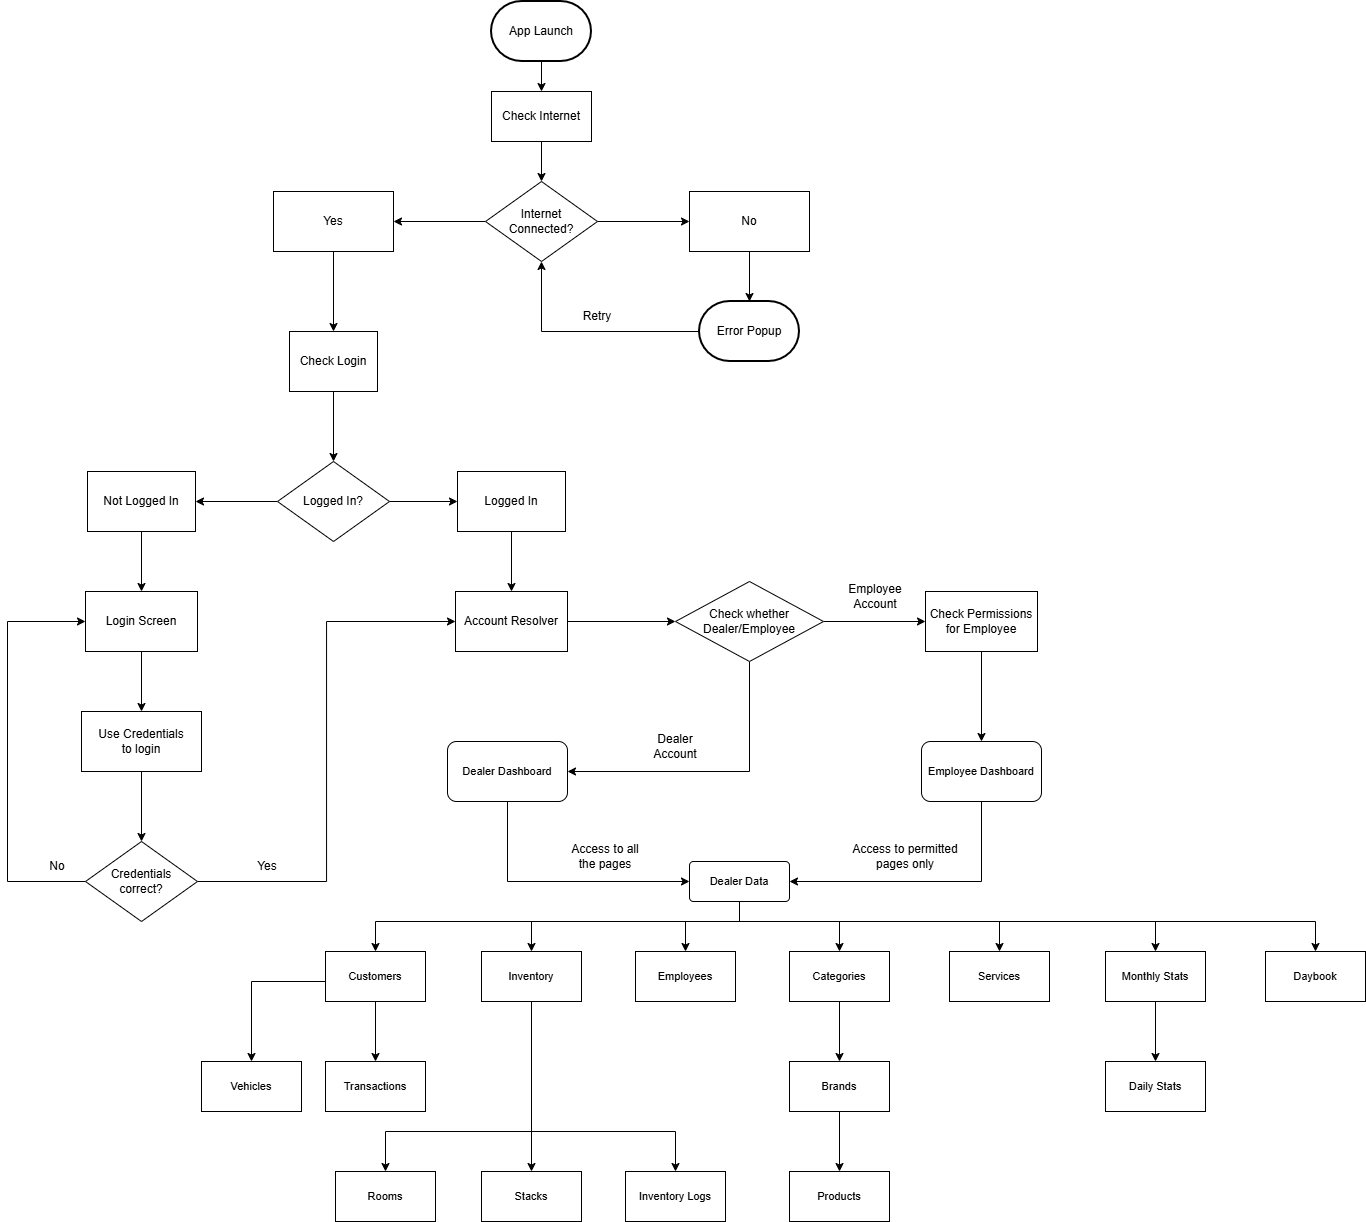
\includegraphics[width=0.85\linewidth]{er_diagram.png}
    \caption{Entity-Relationship Diagram — Trackit}
    \label{fig:er-diagram}
\end{figure}

\subsubsection*{3.5.4 Database Security and Access Control}
\addcontentsline{toc}{subsubsection}{3.5.4 Database Security and Access Control}

Access to all Firestore collections is governed by Firebase Security Rules, which are evaluated server-side before any read or write operation is permitted. The security rules enforce the following access control policies:

\begin{itemize}
    \item Only authenticated users with a valid Firebase session token are permitted to access any collection within the database.
    \item Dealers are granted read and write access exclusively to documents where the \texttt{dealerId} field matches their own Firebase UID, ensuring strict data isolation between different dealer accounts.
    \item Workers are granted access only to the collections corresponding to the modules for which their permission map contains an active grant, as stored in their \texttt{workers} document.
    \item No client-side code is trusted with privilege escalation; all access decisions are enforced at the Firebase backend level, independent of the application layer.
\end{itemize}

\subsection*{3.6 Methodology}
\addcontentsline{toc}{subsection}{3.6 Methodology}

The development methodology for Trackit followed an Agile iterative approach, with structured sprints delivering independently functional modules that were progressively integrated into the complete system. The following table outlines the end-to-end development and deployment workflow adopted for the project:

\renewcommand{\arraystretch}{1.5}
\begin{longtable}{|p{3.8cm}|p{9.8cm}|}
\caption{System Development and Deployment Workflow — Trackit} \label{tab:workflow} \\
\hline
\textbf{Phase} & \textbf{Description} \\
\hline
\endfirsthead
\multicolumn{2}{c}{{\tablename\ \thetable{} -- continued from previous page}} \\
\hline
\textbf{Phase} & \textbf{Description} \\
\hline
\endhead
\hline \multicolumn{2}{|r|}{{Continued on next page}} \\ \hline
\endfoot
\hline
\endlastfoot
Requirement Gathering & Stakeholder discussions with Auribises Technologies to identify business pain points, feature requirements, and system constraints for tyre dealer operations. \\
\hline
System Design & Definition of Firestore collection schema, application architecture, module decomposition, UI wireframing, and permission model design. \\
\hline
Firebase Configuration & Firebase project setup, enabling of Authentication, Firestore, and Hosting services, configuration of security rules, and integration of Firebase SDKs in Flutter and NextJS projects. \\
\hline
Mobile Application Development & Sprint-wise implementation of Flutter modules covering authentication, customer management, inventory management, sales and daybook, reporting, and PDF export. \\
\hline
Web Portal Development & Development of the NextJS dealer portal covering worker account management, permission configuration, and inventory overview. \\
\hline
Integration and Synchronization Testing & Verification of real-time data synchronization across mobile and web clients, validation of role-based access enforcement, and end-to-end functional testing of all modules. \\
\hline
UI Refinement and Dark Mode & Application of final UI polish, implementation of dark mode support, resolution of cross-platform rendering inconsistencies, and accessibility improvements. \\
\hline
Deployment & Production deployment of the NextJS web portal on Vercel and Firebase Hosting; publication of the Flutter mobile application to the Google Play Store and Apple App Store. \\
\hline
Post-Deployment Review & Monitoring of application performance, identification of post-release defects, and collection of stakeholder feedback for future enhancement planning. \\
\hline
\end{longtable}
\newpage
\begin{center}
    \section*{Chapter 4: Implementation, Testing, and Maintenance}
    \addcontentsline{toc}{section}{4. Implementation, Testing, and Maintenance}
\end{center}
\subsection*{4.1 Tools and Technologies Used}
\addcontentsline{toc}{subsection}{4.1 Tools \& Technologies Used}
This project utilizes modern cross-platform and cloud-based technologies for efficient application development, deployment, and real-time data management.
\renewcommand{\arraystretch}{1.4}
\begin{longtable}{|p{4cm}|p{5cm}|p{5cm}|}
\caption{Technology Stack and Purpose} \label{tab:tech-stack} \\
\hline
\textbf{Component} & \textbf{Technology / Tool} & \textbf{Purpose} \\
\hline
\endfirsthead
\multicolumn{3}{c}{{\tablename\ \thetable{} -- continued from previous page}} \\
\hline
\textbf{Component} & \textbf{Technology / Tool} & \textbf{Purpose} \\
\hline
\endhead
\hline \multicolumn{3}{|r|}{{Continued on next page}} \\ \hline
\endfoot
\hline
\endlastfoot
Mobile Application & Flutter & Cross-platform mobile application development for Android and iOS \\
\hline
Web Portal & NextJS & Development of the dealer management web portal \\
\hline
Backend Services & Firebase & Authentication, database management, cloud synchronization, and hosting \\
\hline
Database & Firestore & Real-time cloud database for storing customer, inventory, and sales data \\
\hline
Authentication & Firebase Authentication & Secure login system using email and password \\
\hline
Hosting Platform & Vercel, Firebase Hosting & Deployment and hosting of web applications and backend services \\
\hline
Mobile App Deployment & Google Play Store, Apple App Store & Distribution of the mobile application \\
\hline
IDE & Android Studio, VS Code, Antigravity & Application development, testing, and debugging \\
\hline
Version Control & Git, GitHub & Source code management and collaboration \\
\hline
State Management & Custom db\_provider & Managing application state and database synchronization \\
\hline
PDF Generation & Flutter Packages: pdf, printing & Generating and exporting transaction PDFs \\
\hline
Charts and Analytics & Flutter Package: fl\_chart & Displaying sales and inventory analytics visually \\
\hline
\end{longtable}

\subsection*{4.2 Coding Standards}
\addcontentsline{toc}{subsection}{4.2 Coding Standards}
The project follows standard coding guidelines for Flutter, Firebase, and web development, focusing on readability, modularity, maintainability, and secure application development.\\[0.25cm]
\textbf{Key Practices Followed:}
\begin{itemize}
    \item \textbf{Feature-Based Modular Structure:} The application is organized into separate modules for inventory, customer management, sales, and reports. Different directories are maintained for screens, services, models, providers, themes, and reusable widgets for better scalability and maintenance.
    \item \textbf{Descriptive Naming Conventions:} Screen file names follow snake\_case formatting, directory names use camelCase, and class names follow PascalCase notation to maintain consistency and code readability.
    \item \textbf{Centralized State Management:} The project uses custom providers such as db\_provider, theme\_provider, and an account resolver module to handle application state, theme management, authentication, and permission-based navigation efficiently.
    \item \textbf{Reusable UI Components:} A common widgets directory and centralized theme management system are used to maintain consistent UI design, reusable components, and standardized color schemes across the application.
    \item \textbf{Centralized Error Handling:} Error management is handled through a dedicated module located in lib/assets/core/errors, ensuring consistent handling of exceptions and application-level errors.
    \item \textbf{Version Control and Collaboration:} Git and GitHub are used for source code management, regular code synchronization, and collaborative development.
    \item \textbf{Security Practices:} Firebase Authentication rules and role-based validation are implemented to ensure secure access control and restricted page access for employees based on assigned permissions.
\end{itemize}

\subsection*{4.3 Project Scheduling}
\addcontentsline{toc}{subsection}{4.3 Project Scheduling}
The development of Trackit was carried out in multiple phases during the semester training period from January to June.
\begin{longtable}{|p{4cm}|p{10cm}|}
\caption{Development Phases and Description} \label{tab:project-scheduling} \\
\hline
\textbf{Phase} & \textbf{Description} \\
\hline
\endfirsthead
\multicolumn{2}{c}%
{{\tablename\ \thetable{} -- continued from previous page}} \\
\hline
\textbf{Phase} & \textbf{Description} \\
\hline
\endhead
\hline \multicolumn{2}{|r|}{{Continued on next page}} \\ \hline
\endfoot
\hline
\endlastfoot
Requirement Analysis & Initial project requirements, UI/UX planning, and database structure were provided by Auribises based on tyre dealer business requirements. \\
\hline
Authentication Module & A basic Firebase Authentication system was first implemented to verify login functionality and user access. \\
\hline
Role-Based Access System & A permission-based access system was later integrated to support dealer and employee roles according to updated project requirements. \\
\hline
Customer \& Inventory Modules & Customer management and Room-Stack Inventory Management modules were developed simultaneously. \\
\hline
Sales \& Reporting Module & Sales tracking, transaction management, PDF export, inventory logs, and reporting functionalities were implemented. \\
\hline
Testing Phase & Continuous testing was performed using small datasets and later through partial migration of data from the previous Madhok Enterprises application. \\
\hline
Deployment Phase & Deployment is currently in progress while business data migration and client review meetings are being conducted before Play Store and App Store release. \\
\hline
\end{longtable}

\subsubsection*{4.3.1 Project Duration}
\addcontentsline{toc}{subsubsection}{4.3.1 Project Duration}
\begin{itemize}
    \item \textbf{Training Duration:} January – June
    \item \textbf{Development Approach:} Phase-wise iterative development
    \item \textbf{Project Type:} Team Project\\[1cm]
\end{itemize}
\subsubsection*{4.3.2 Team Responsibilities}
\addcontentsline{toc}{subsubsection}{4.3.2 Team Responsibilities}

\begin{longtable}{|p{5cm}|p{9cm}|}
\caption{Team Responsibilities} \label{tab:team-responsibilities} \\
\hline
\textbf{Team Member} & \textbf{Responsibility} \\
\hline
\endfirsthead
\multicolumn{2}{c}%
{{\tablename\ \thetable{} -- continued from previous page}} \\
\hline
\textbf{Team Member} & \textbf{Responsibility} \\
\hline
\endhead
\hline \multicolumn{2}{|r|}{{Continued on next page}} \\ \hline
\endfoot
\hline
\endlastfoot
Arshdeep Kaur & Development of NextJS Web Portal \\
\hline
Aarchie Maggu & Flutter Mobile Application Development \\
\hline
Brahamjot Singh & Flutter Mobile Application Development \\
\hline
\end{longtable}

\subsubsection*{4.3.3 Detailed Development Phases}
\addcontentsline{toc}{subsubsection}{4.3.3 Detailed Development Phases}

\textbf{4.3.3.1 Requirement Analysis}

\begin{itemize}
    \item Understanding the business workflow and operational challenges faced by tyre dealers.
    
    \item Initial project requirements, UI/UX design concepts, and database structure were provided by Auribises.
    
    \item Existing Madhok Enterprises application and dealer requirements were analyzed for system planning.
    
    \item Focus was placed on developing a scalable and centralized system for inventory, customer, and sales management.
\end{itemize}

\textbf{4.3.3.2 Authentication Module Development}

\begin{itemize}
    \item A basic authentication system was implemented using Firebase Authentication.
    
    \item Email and password login functionality was developed for secure user access.
    
    \item Initial authentication testing was performed to verify login validation and session handling.
    
    \item This phase established the foundation for user management and application security.
\end{itemize}

\textbf{4.3.3.3 Role-Based Access System}

\begin{itemize}
    \item A permission-based access system was introduced according to updated project requirements.
    
    \item The application checks whether the logged-in account belongs to a dealer or employee collection in Firestore.
    
    \item Employees are granted access only to modules and pages permitted by the dealer.
    
    \item Role-based validation was implemented to improve operational security and access control.
\end{itemize}

\textbf{4.3.3.4 Customer and Inventory Modules}

\begin{itemize}
    \item Customer Management and Inventory Management modules were developed simultaneously.
    
    \item Customer records, vehicle-wise transaction history, and warranty-related information were implemented.
    
    \item The Room-Stack Inventory Management System was developed for organized stock handling.
    
    \item Inventory tracking and stock movement logging features were integrated for better inventory management.
\end{itemize}

\textbf{4.3.3.5 Sales and Reporting Module}

\begin{itemize}
    \item Sales management functionality was implemented for transaction creation and inventory deduction.
    
    \item Cart-based sales logging and customer transaction tracking were integrated into the application.
    
    \item PDF export functionality was added for sharing customer transaction details.
    
    \item Reporting features such as inventory logs and daily sales reports were implemented for business analysis.
\end{itemize}

\textbf{4.3.3.6 Testing Phase}

\begin{itemize}
    \item Continuous testing was performed throughout the development lifecycle.
    
    \item Initial testing was conducted using small datasets to verify module functionality.
    
    \item Partial migration of data from the previous Madhok Enterprises application was performed for compatibility testing.
    
    \item Application performance, data synchronization, and operational behavior were validated during testing.
\end{itemize}

\textbf{4.3.3.7 Deployment Phase}

\begin{itemize}
    \item The deployment phase is currently in progress.
    
    \item Existing business data from the previous Madhok Enterprises application is being migrated into Trackit.
    
    \item Regular client review meetings are being conducted for functionality verification and approval.
    
    \item After successful validation, the application will be deployed on the Google Play Store and Apple App Store.
\end{itemize}

\subsection*{4.4 Testing Techniques}
\addcontentsline{toc}{subsection}{4.4 Testing Techniques}

\subsubsection*{4.4.1 Testing Strategy}
\addcontentsline{toc}{subsubsection}{4.4.1 Testing Strategy}
The Trackit application was tested continuously during development to ensure proper functionality, security, role-based access control, inventory management, sales processing, PDF generation, and real-time Firestore synchronization. Testing was performed using emulators, real devices, browsers, and Firebase tools to validate both normal operations and edge case scenarios across multiple platforms.
\renewcommand{\arraystretch}{1.4}
\begin{longtable}{|p{4cm}|p{10cm}|}
\caption{Testing Levels and Descriptions} \label{tab:testing-levels} \\
\hline
\textbf{Level} & \textbf{Description} \\
\hline
\endfirsthead
\multicolumn{2}{c}%
{{\tablename\ \thetable{} -- continued from previous page}} \\
\hline
\textbf{Level} & \textbf{Description} \\
\hline
\endhead
\hline \multicolumn{2}{|r|}{{Continued on next page}} \\ \hline
\endfoot
\hline
\endlastfoot
Authentication Testing & Login validation was tested using correct and incorrect credentials to verify secure authentication and error handling. \\
\hline
Permission Testing & Employee permissions were tested by modifying access rights and verifying restricted module accessibility. \\
\hline
Inventory Testing & Inventory addition, stock updates, stock deduction, and Room-Stack inventory management were tested. \\
\hline
Sales Flow Testing & End-to-end sales flow including cart management, transaction creation, and inventory deduction was validated. \\
\hline
PDF Export Testing & Customer transaction PDF export functionality was tested for successful document generation and sharing. \\
\hline
Real-Time Synchronization Testing & Firestore synchronization and real-time updates across devices and platforms were tested successfully. \\
\hline
UI Testing & Dark mode, responsive layouts, reusable widgets, and overall user interface consistency were tested across platforms. \\
\hline
Cross-Platform Testing & Application functionality was tested on Android Emulator, iOS Simulator, real Android devices, and web browsers. \\
\hline
Error Handling Testing & Invalid login, out-of-stock conditions, internet connectivity checks, and unauthorized access scenarios were tested. \\
\hline
\end{longtable}

\subsubsection*{4.4.2 Testing Tools Used}
\addcontentsline{toc}{subsubsection}{4.4.2 Testing Tools Used}
\begin{itemize}
    \item Android Emulator for Android application testing.
    \item iOS Simulator for iOS compatibility testing.
    \item Real Android devices for real-world application testing.
    \item Chrome browser for web application testing.
    \item Firebase Console for database monitoring and synchronization testing.
    \item Debug console logs for identifying and resolving runtime issues.
\end{itemize}

\subsubsection*{4.4.3 Error and Edge Case Testing}
\addcontentsline{toc}{subsubsection}{4.4.3 Error and Edge Case Testing}
\begin{itemize}
    \item Invalid login attempts display authentication errors and prevent unauthorized access.
    \item Out-of-stock conditions are detected and displayed to the user.
    \item Internet connectivity is checked during application startup, and appropriate error messages are shown if connectivity is unavailable.
    \item Unauthorized page access is restricted through role-based validation and Firebase security rules.
\end{itemize}

\subsection*{4.5 Test Cases used in the Project}
\addcontentsline{toc}{subsection}{4.5 Test Cases used in the Project}
The following test cases were used to validate the functionality, security, and operational workflow of the Trackit application. The testing process ensured that all major modules operated correctly under both normal and edge case conditions.
\begin{longtable}{|p{2cm}|p{4cm}|p{6cm}|p{2cm}|}
\caption{Test Cases Used in the Project} \label{tab:test-cases} \\
\hline
\textbf{Test ID} & \textbf{Test Scenario} & \textbf{Expected Result} & \textbf{Status} \\
\hline
\endfirsthead
\multicolumn{4}{c}%
{{\tablename\ \thetable{} -- continued from previous page}} \\
\hline
\textbf{Test ID} & \textbf{Test Scenario} & \textbf{Expected Result} & \textbf{Status} \\
\hline
\endhead
\hline \multicolumn{4}{|r|}{{Continued on next page}} \\ \hline
\endfoot
\hline
\endlastfoot
TC-01 & Dealer Login Validation & Dealer should successfully log in using valid email and password credentials. & Passed \\
\hline
TC-02 & Invalid Login Attempt & System should display authentication error and deny access for invalid credentials. & Passed \\
\hline
TC-03 & Employee Permission Validation & Employee should access only the modules permitted by the dealer. & Passed \\
\hline
TC-04 & Inventory Addition & Newly added inventory should update correctly in the Room-Stack inventory system. & Passed \\
\hline
TC-05 & Out of Stock Validation & System should display out-of-stock message when inventory is unavailable. & Passed \\
\hline
TC-06 & Sales Transaction Creation & Sales transaction should update customer history and reduce inventory quantity. & Passed \\
\hline
TC-07 & PDF Export Functionality & Customer transaction should be successfully exported as a PDF document. & Passed \\
\hline
TC-08 & Real-Time Firestore Synchronization & Changes made on one device should reflect across all connected devices in real time. & Passed \\
\hline
TC-09 & Dark Mode Testing & Application theme should switch correctly between light and dark mode. & Passed \\
\hline
TC-10 & Internet Connectivity Check & Application should display an error message when internet connectivity is unavailable. & Passed \\
\hline
TC-11 & Unauthorized Access Validation & Unauthorized users should not be allowed to access restricted modules or pages. & Passed \\
\hline
TC-12 & Inventory Log Tracking & Inventory logs should correctly display stock additions and stock deductions. & Passed \\
\hline
\end{longtable}


\newpage
\begin{center}
    \section*{Chapter 5: Contribution to Sustainable Development Goals}
    \addcontentsline{toc}{section}{5. Contribution to Sustainable Development Goals}
\end{center}

\vspace{0.8em}

\textbf{SDG 8 – Decent Work and Economic Growth} \\
\textit{Promote sustained, inclusive and sustainable economic growth, full and productive employment and decent work for all.}

\begin{itemize}
    \item \textbf{Improves Business Efficiency:} Trackit reduces manual paperwork and simplifies inventory, customer, and sales management for tyre dealers through a centralized digital platform.
    \item \textbf{Enhances Employee Coordination:} The role-based access system allows dealers to manage employee responsibilities efficiently while improving workflow organization.
    \item \textbf{Supports Small and Large Businesses:} The system is designed for both small retailers and large tyre dealers, helping businesses digitally manage operations and improve productivity.
    \item \textbf{Reduces Operational Errors:} Real-time synchronization and centralized data storage minimize stock mismatches and errors in customer record management.
\end{itemize}
\textbf{SDG 9 – Industry, Innovation and Infrastructure} \\
\textit{Build resilient infrastructure, promote inclusive and sustainable industrialization and foster innovation.}
\begin{itemize}
    \item \textbf{Promotes Digital Transformation:} Trackit introduces a cloud-based SaaS platform for modernizing traditional tyre business operations.
    \item \textbf{Real-Time Cloud Synchronization:} The system provides synchronized access to inventory, sales, and customer data across multiple devices and locations using Firebase services.
    \item \textbf{Cross-Platform Accessibility:} The application is available on Android, iOS, and web platforms, making business management more flexible and accessible.
    \item \textbf{Innovative Inventory Management:} The Room-Stack Inventory Management System provides a structured approach for organizing and tracking tyre inventory efficiently.
\end{itemize}
\textbf{SDG 12 – Responsible Consumption and Production} \\
\textit{Ensure sustainable consumption and production patterns.}
\begin{itemize}
    \item \textbf{Efficient Inventory Utilization:} The system helps dealers maintain accurate inventory records and reduces stock mismanagement and unnecessary wastage.
    \item \textbf{Reduces Paper-Based Documentation:} Digital storage of customer records, invoices, and transaction history decreases dependency on manual paperwork.
    \item \textbf{Improves Warranty Tracking:} Organized customer and vehicle transaction records help dealers efficiently manage warranty-related claims and tyre replacement history.
    \item \textbf{Digital Report Generation:} Features such as PDF export and inventory logs promote systematic record maintenance and better resource management.
\end{itemize}

\textbf{Summary:} \\
Trackit contributes to multiple Sustainable Development Goals by promoting digital business management, operational efficiency, and organized inventory handling in the tyre retail industry. The system supports economic growth, technological innovation, and responsible resource utilization through its cloud-based architecture, real-time synchronization, and centralized management features.

\newpage
\begin{center}
    \section*{Chapter 6: Results and Discussions}
\end{center}
\addcontentsline{toc}{section}{6. Results \& Discussions}

\subsection*{6.1 Results Overview}
\addcontentsline{toc}{subsection}{6.1 Results Overview}

The Trackit system was successfully developed and validated across all planned modules. The
following outcomes were observed upon completion of development, integration testing, and
cross-platform deployment:

\begin{itemize}
    \item The authentication and role identification workflow functioned correctly for both dealer
    and worker accounts, with permission-based navigation enforced consistently across all
    modules.
    \item The Room-Stack Inventory Management System enabled accurate organization, addition,
    and retrieval of tyre stock, with all operations reflected in real time across connected
    devices.
    \item The cart-based sales logging workflow successfully recorded transactions, updated
    inventory quantities, and generated corresponding daybook entries without data conflicts
    under concurrent access conditions.
    \item Customer search operations returned accurate results within acceptable response times
    for both name-based and contact number-based queries.
    \item PDF export of customer transaction records rendered correctly and completely on both
    Android and iOS devices, producing print-ready documents suitable for billing and record
    maintenance.
    \item Real-time synchronization between the mobile application and the web portal was
    confirmed, with data updates reflecting across all connected clients within the specified
    threshold.
    \item Role-based access control was validated across multiple worker permission configurations,
    with no unauthorized module access observed during testing.
\end{itemize}

\subsection*{6.2 User Interface Representation}
\addcontentsline{toc}{subsection}{6.2 User Interface Representation}

The user interface of Trackit has been designed for operational efficiency and ease of use
in a fast-paced retail environment. The mobile application adopts a clean, drawer-based
navigation structure providing quick access to all primary modules, while the NextJS web
portal employs a sidebar layout suited for desktop-based dealer administration. Both
interfaces support light and dark display modes.

\renewcommand{\arraystretch}{1.4}
\begin{longtable}{|p{4cm}|p{10cm}|}
\caption{Software Modules and Descriptions} \label{tab:software-modules} \\
\hline
\textbf{Module} & \textbf{Description} \\
\hline
\endfirsthead
\multicolumn{2}{c}%
{{\bfseries \tablename\ \thetable{} -- continued from previous page}} \\
\hline
\textbf{Module} & \textbf{Description} \\
\hline
\endhead
\hline \multicolumn{2}{|r|}{{Continued on next page}} \\ \hline
\endfoot
\hline
\endlastfoot
Authentication Module & Handles Firebase-based login with email and password, identifies
dealer or worker role on successful authentication, and enforces
permission-based navigation. \\
\hline
Customer Management Module & Provides customer addition, editing, and search functionality with
vehicle-wise transaction history and warranty portal access. \\
\hline
Inventory Management Module & Implements the Room-Stack structure for organizing tyre stock with
support for addition, adjustment, removal, and inventory log
generation. \\
\hline
Sales and Daybook Module & Manages cart-based sales logging, transaction confirmation,
automatic daybook entry generation, and daily sales summaries. \\
\hline
Reporting and Export Module & Generates visual sales and inventory analytics using
\texttt{fl\_chart} and supports PDF export of individual customer
transactions. \\
\hline
Web Portal — Worker Management & Allows dealers to create worker accounts, assign module-level
permissions, and manage employee access through the NextJS
portal. \\
\hline
Web Portal — Inventory Overview & Provides a consolidated view of inventory across all rooms and
stacks with stock level indicators and management controls. \\
\hline
\end{longtable}

\subsection*{6.3 Snapshots}
\addcontentsline{toc}{subsection}{6.3 Snapshots}

The following screenshots illustrate the key screens of the Trackit mobile application and
web portal as observed during functional testing and validation.

% ---------------------------------------------------------------
%  Paste your actual screenshots below.
% ---------------------------------------------------------------

\begin{figure}[H]
    \centering
    \begin{minipage}{0.22\textwidth}
        \centering
        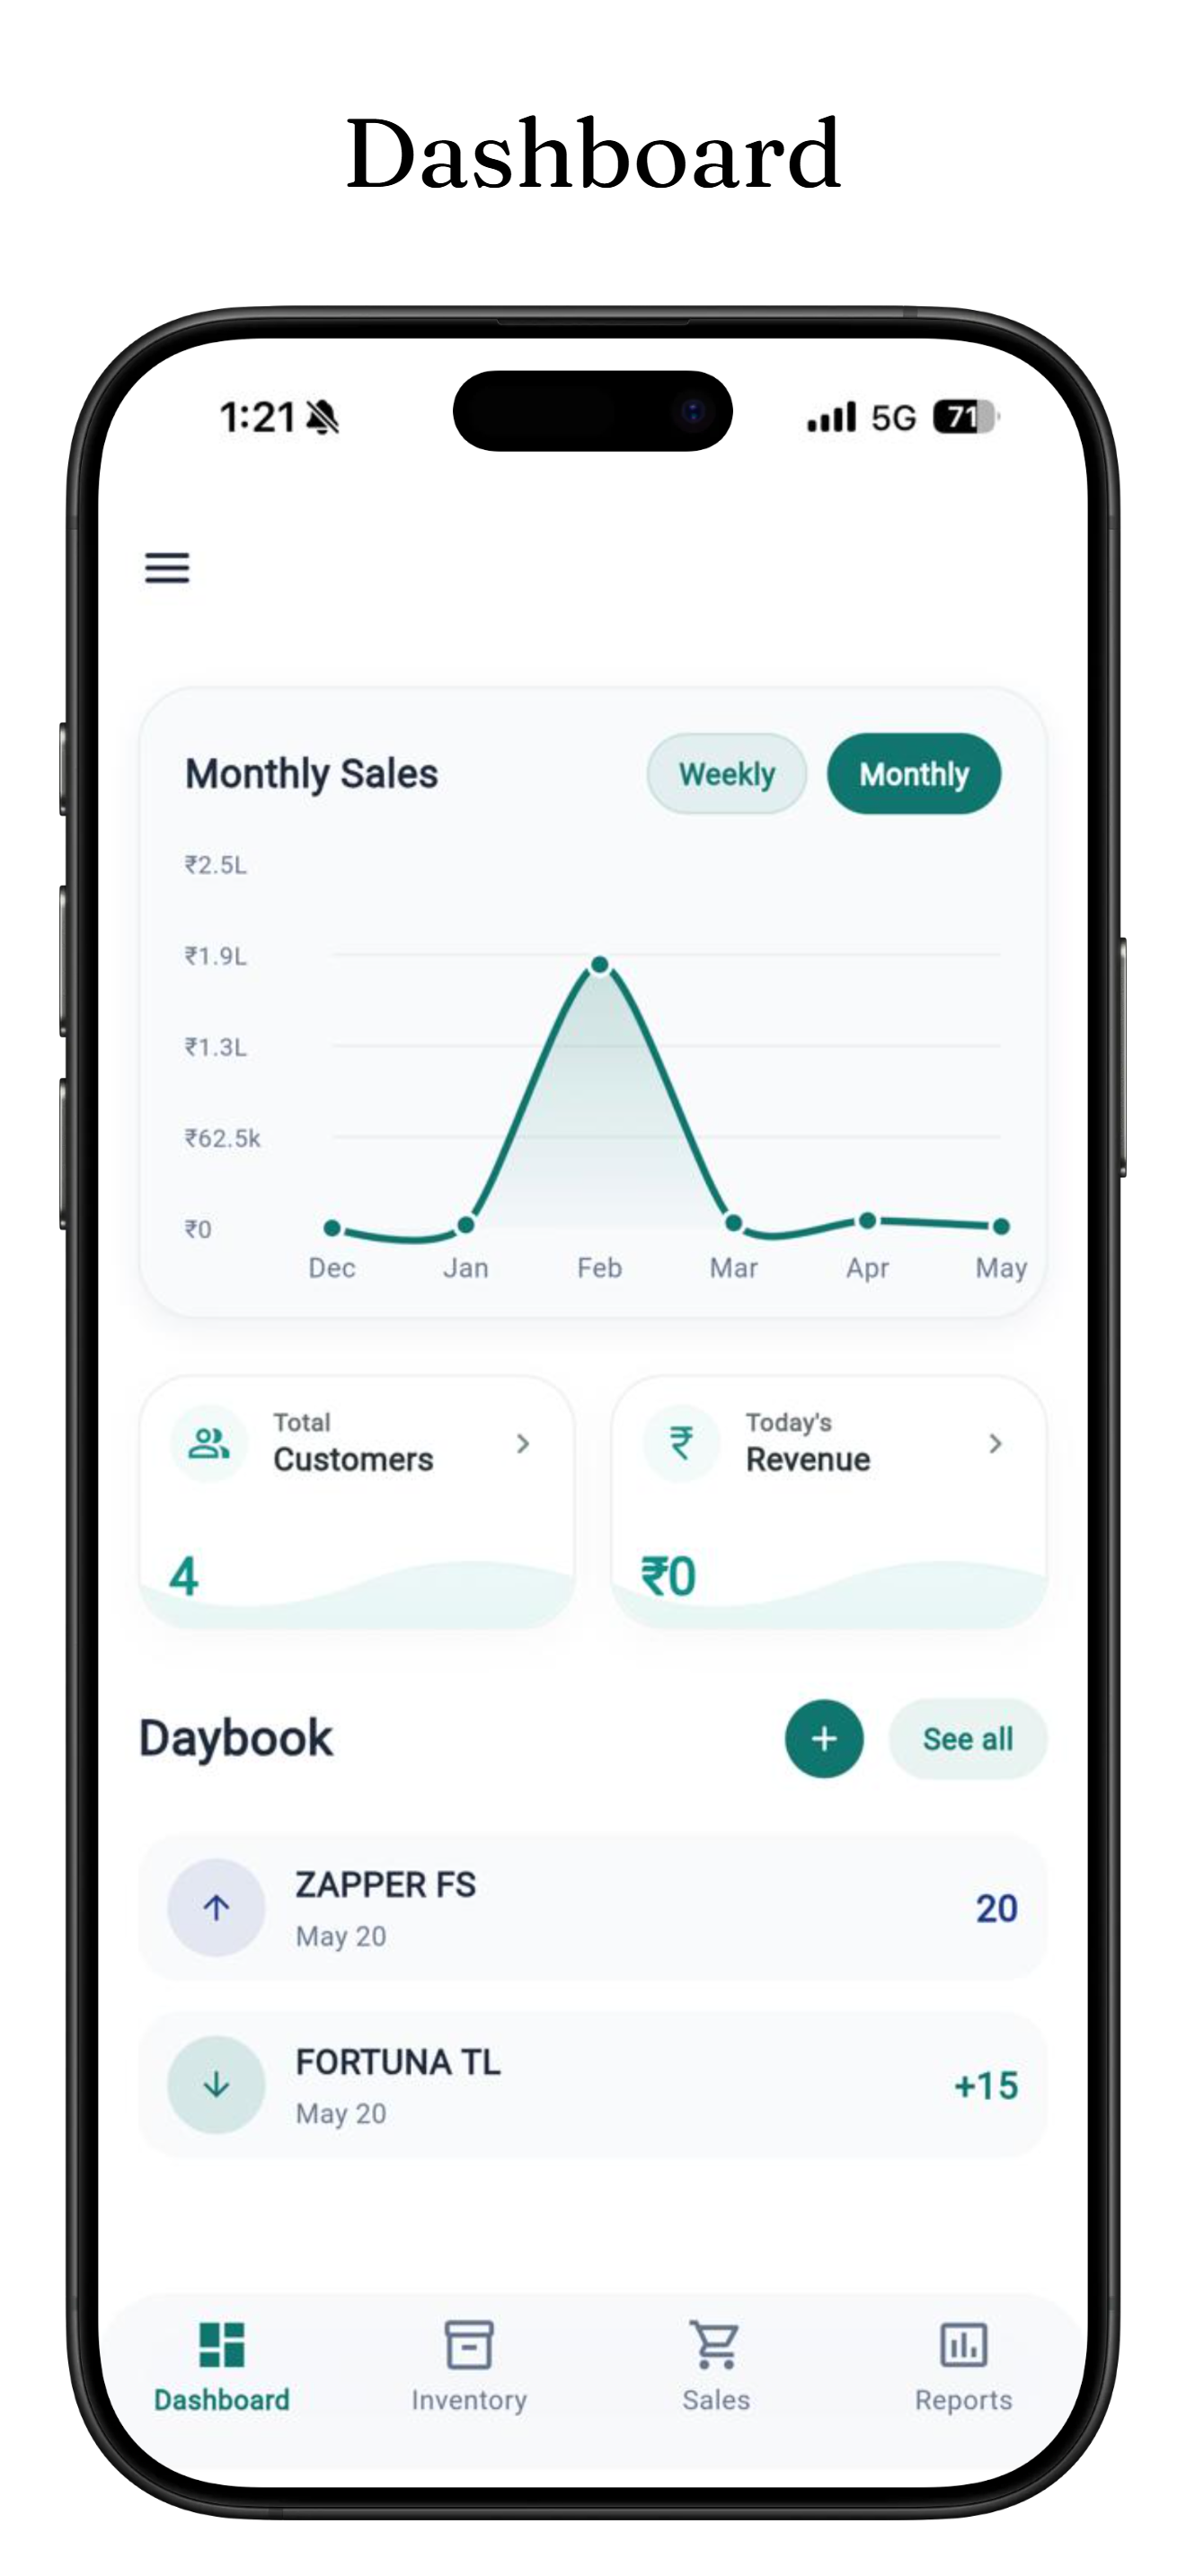
\includegraphics[width=\linewidth]{dashboard.png}
        \caption{Dashboard}
        \label{fig:dashboard}
    \end{minipage}\hfill
    \begin{minipage}{0.22\textwidth}
        \centering
        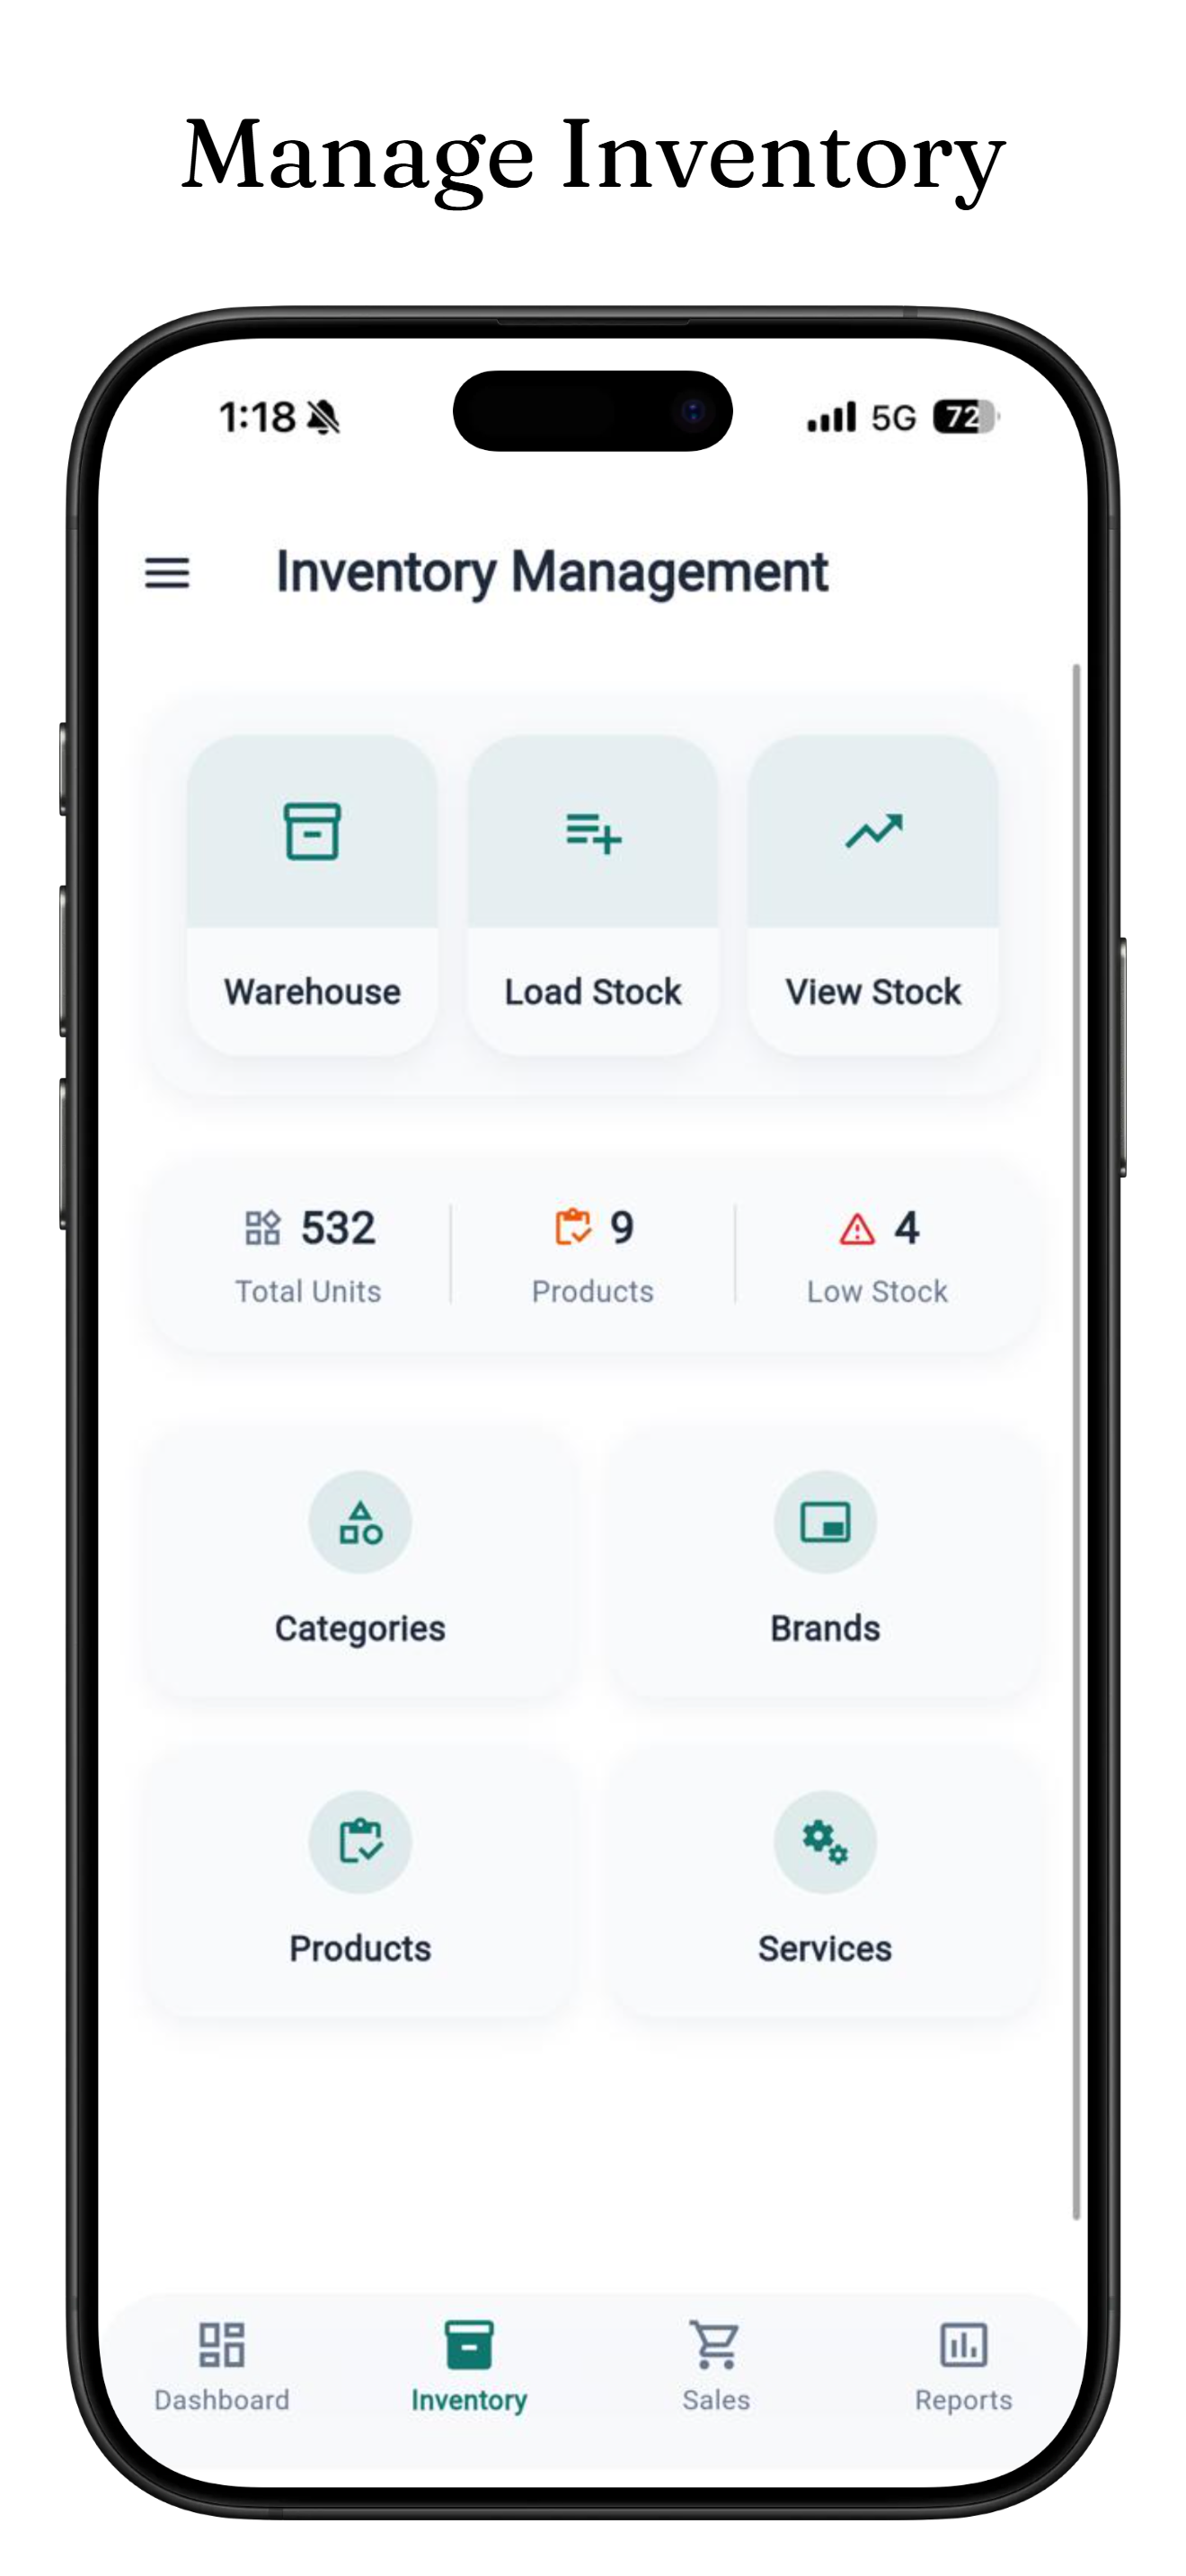
\includegraphics[width=\linewidth]{inventory_management.png}
        \caption{Inventory Management}
        \label{fig:inventory_mgmt}
    \end{minipage}\hfill
    \begin{minipage}{0.22\textwidth}
        \centering
        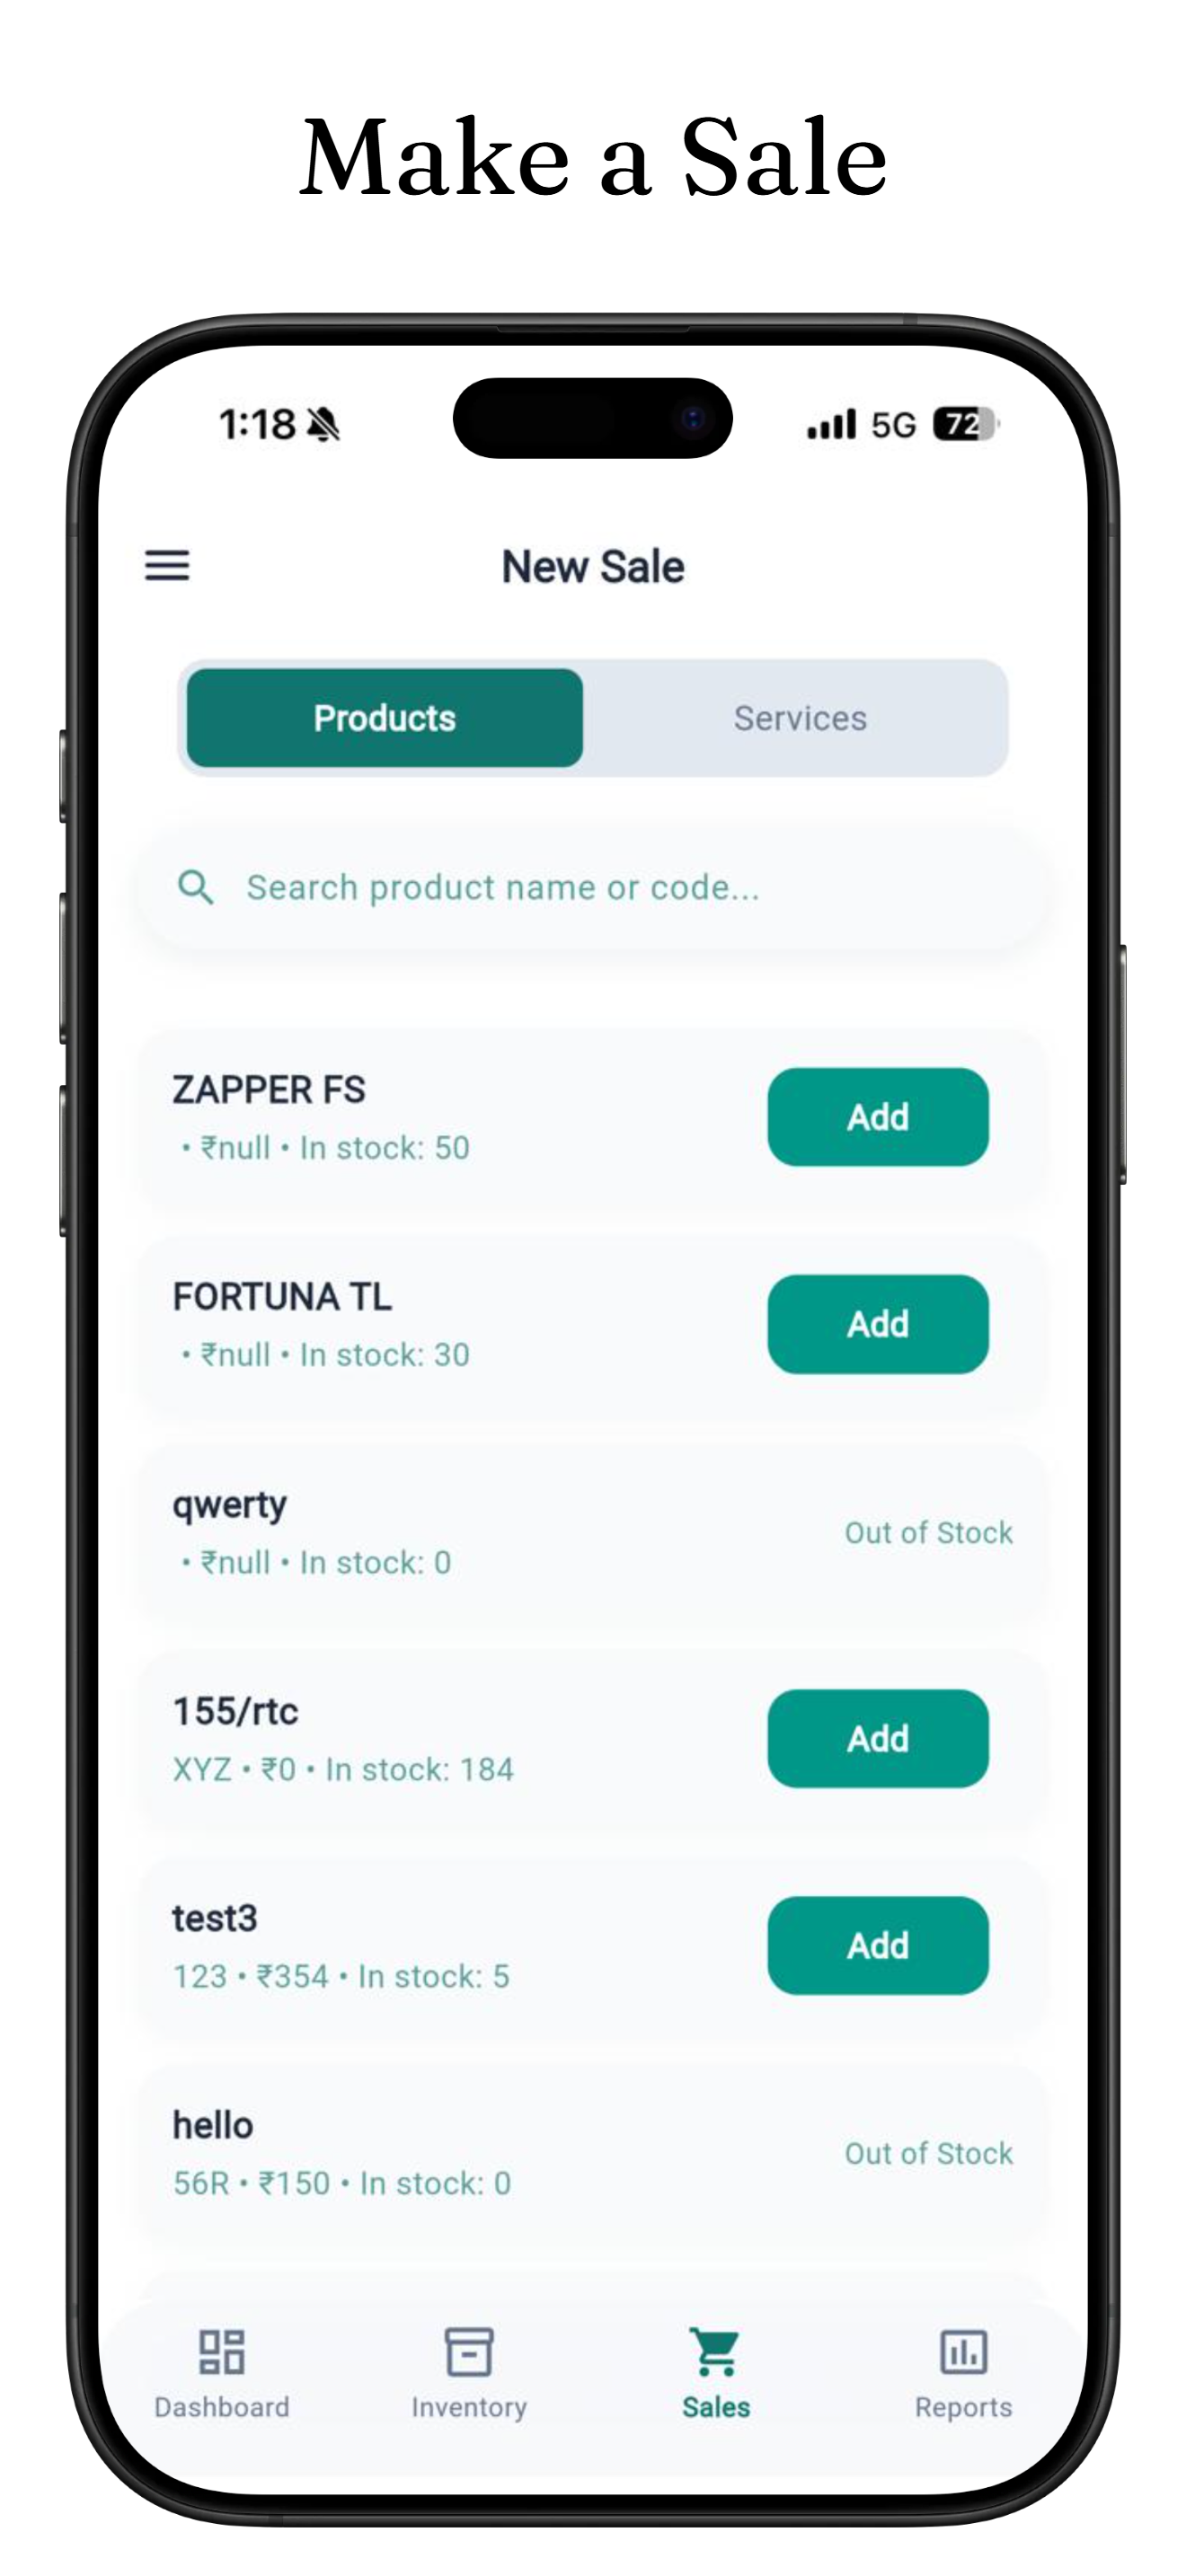
\includegraphics[width=\linewidth]{sales_screen.png}
        \caption{Sales Screen}
        \label{fig:sales_cart}
    \end{minipage}
    \caption{Dashboard, Inventory, and Sales Screens}
    \label{fig:screens_set1}
\end{figure}

\begin{figure}[H]
    \centering
    \begin{minipage}{0.22\textwidth}
        \centering
        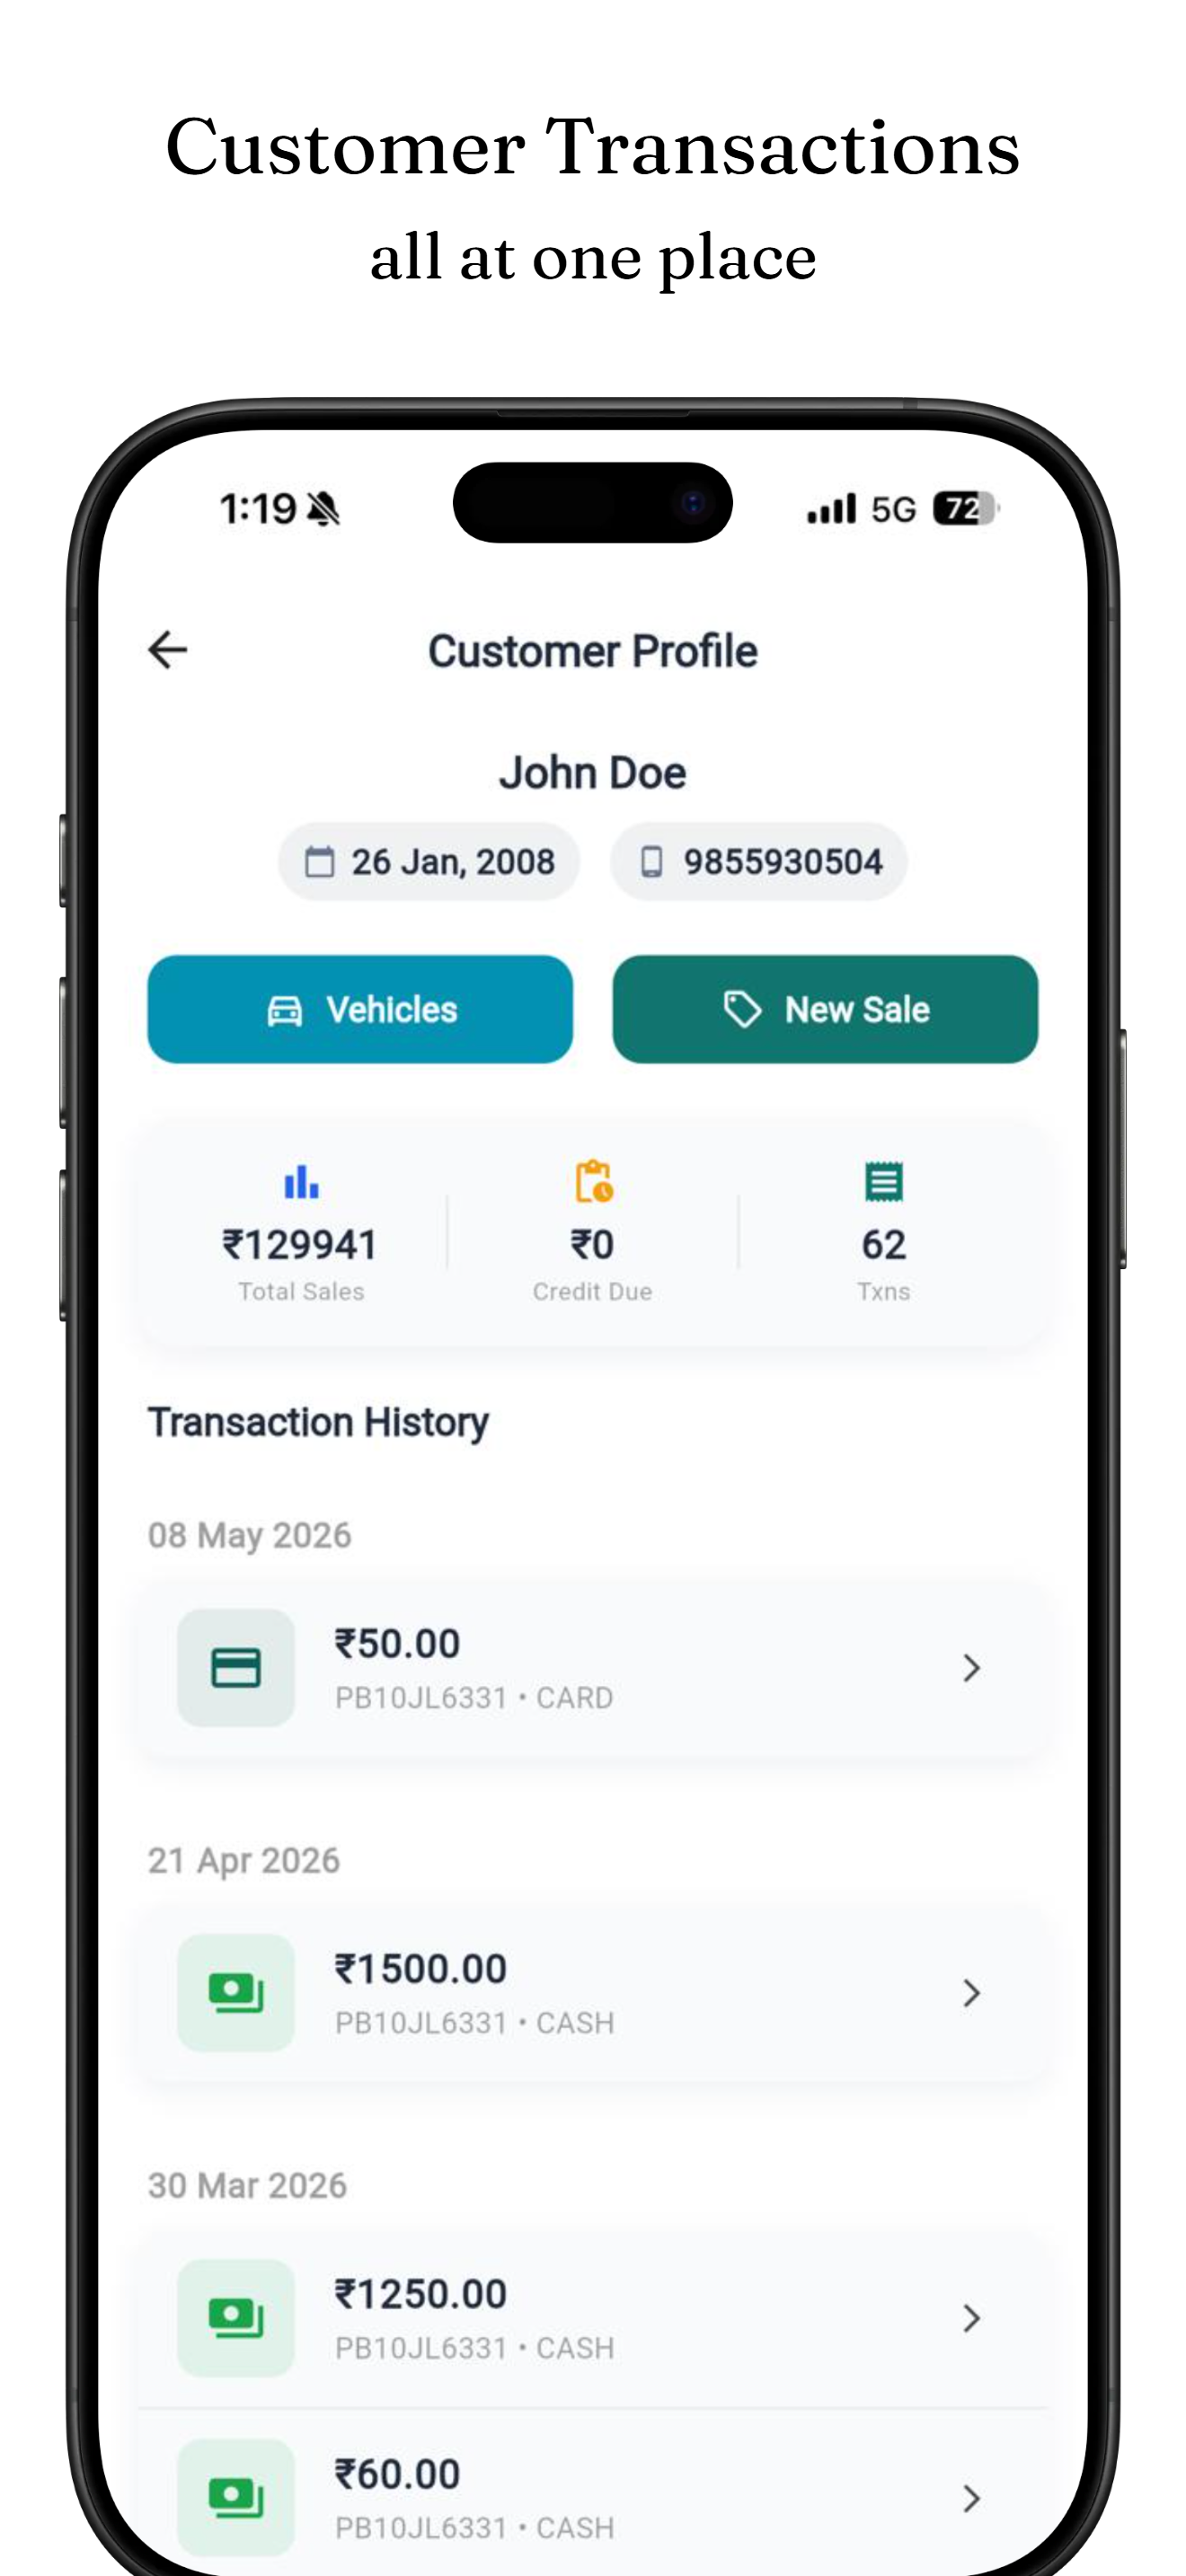
\includegraphics[width=\linewidth]{customer_management.png}
        \caption{Customer Management}
        \label{fig:customer_mgmt}
    \end{minipage}\hfill
    \begin{minipage}{0.22\textwidth}
        \centering
        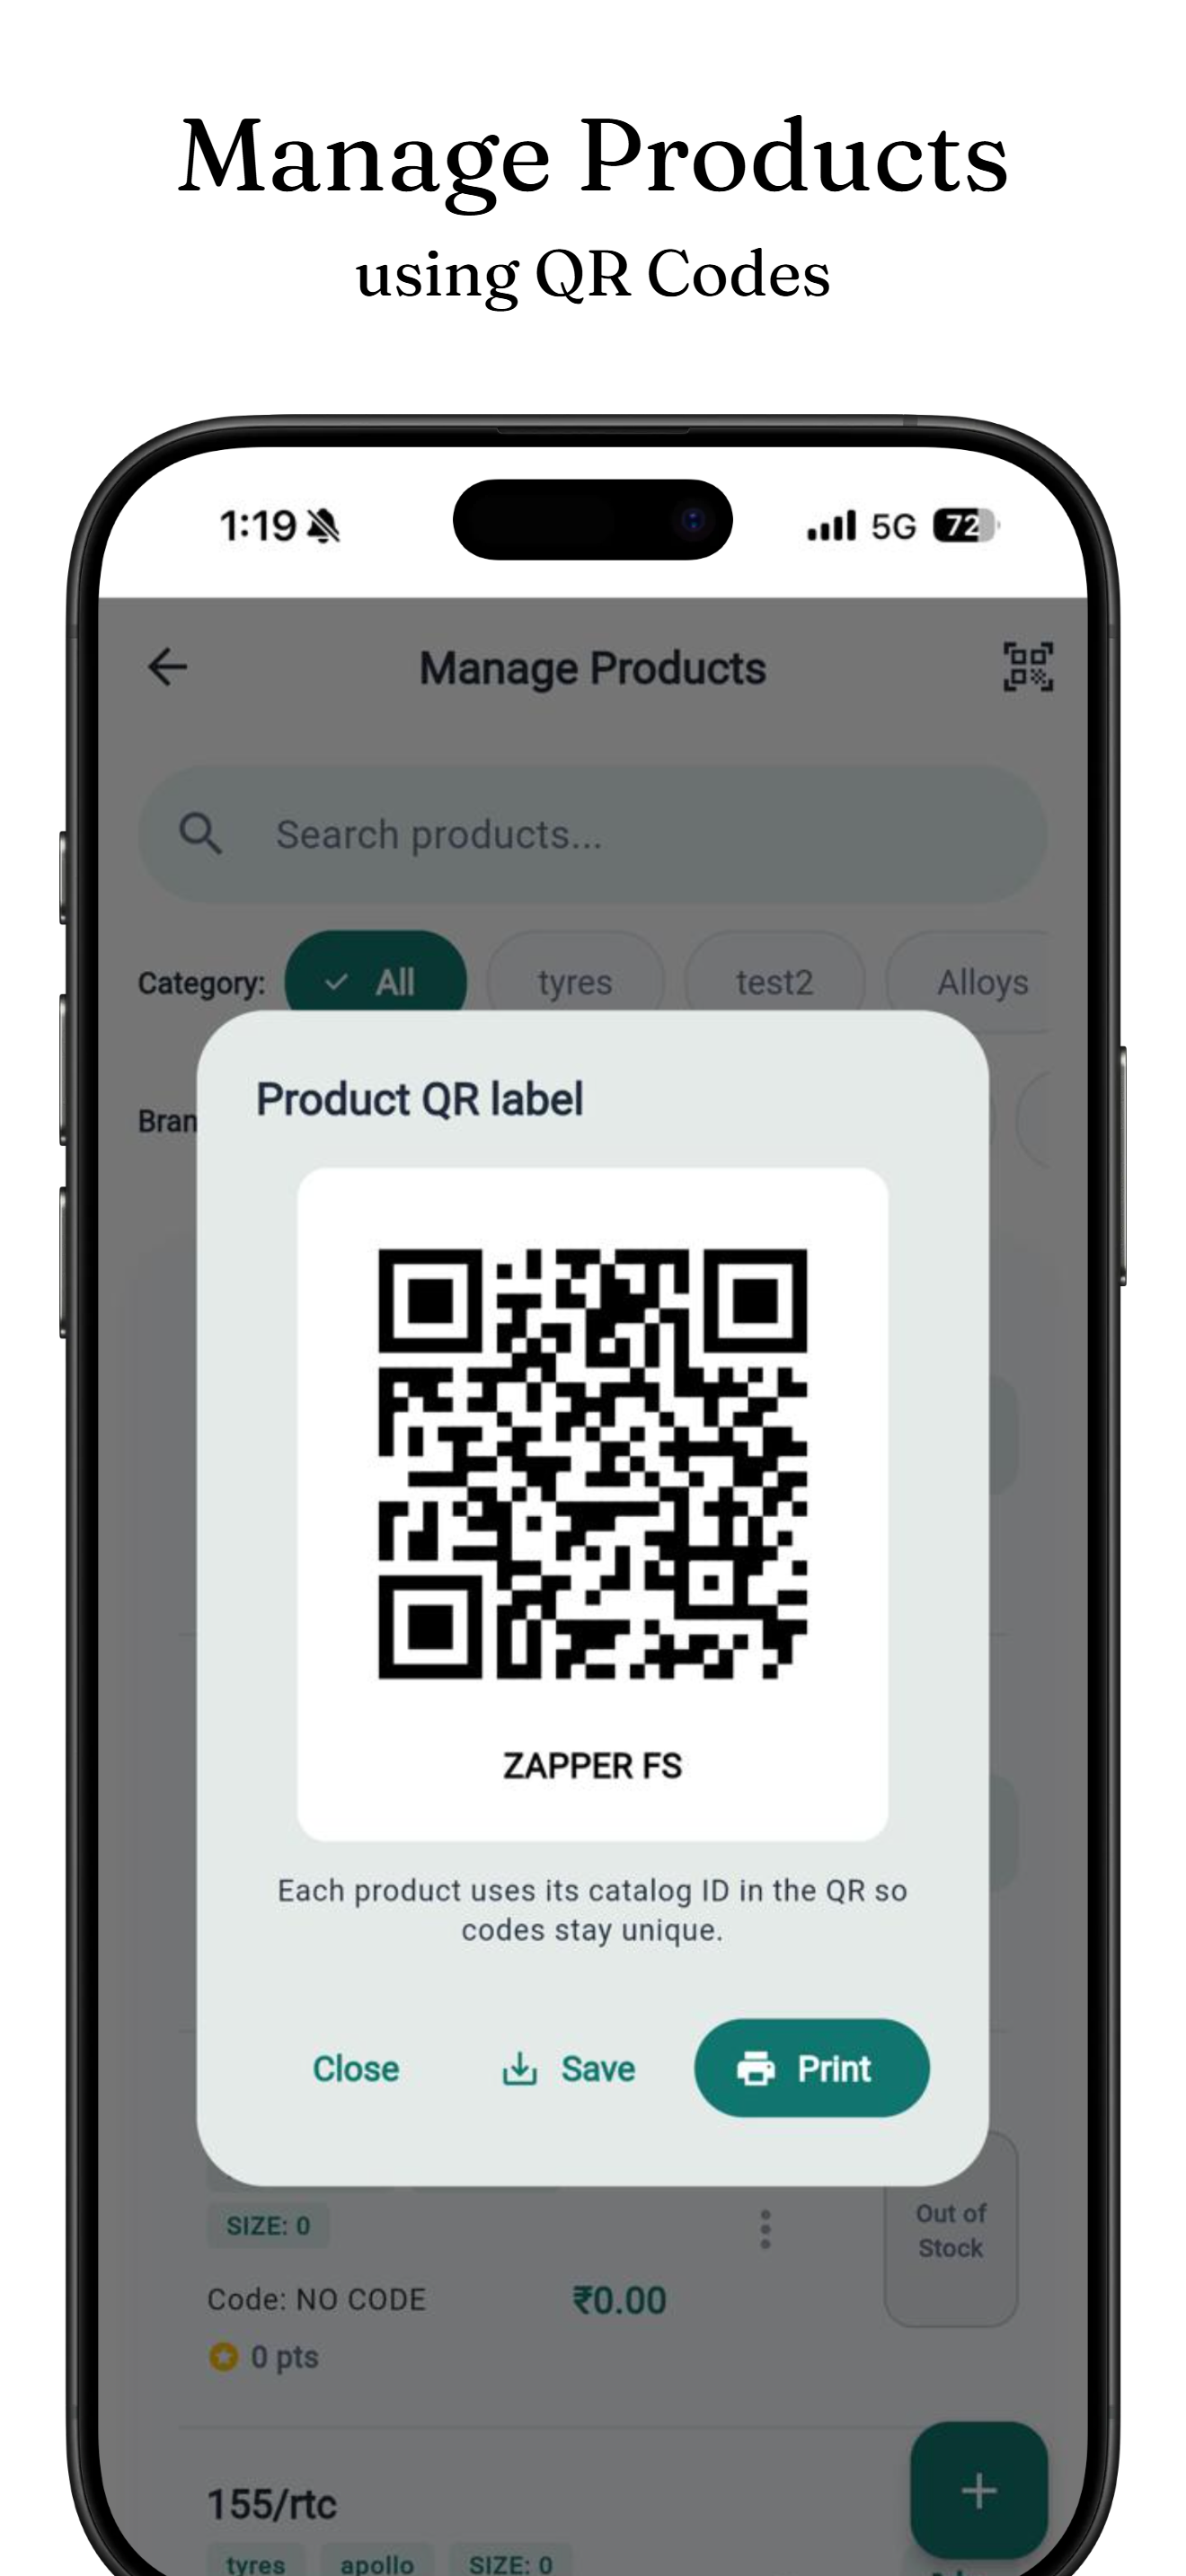
\includegraphics[width=\linewidth]{qr.png}
        \caption{QR Scanner}
        \label{fig:qr_scanner}
    \end{minipage}\hfill
    \begin{minipage}{0.22\textwidth}
        \centering
        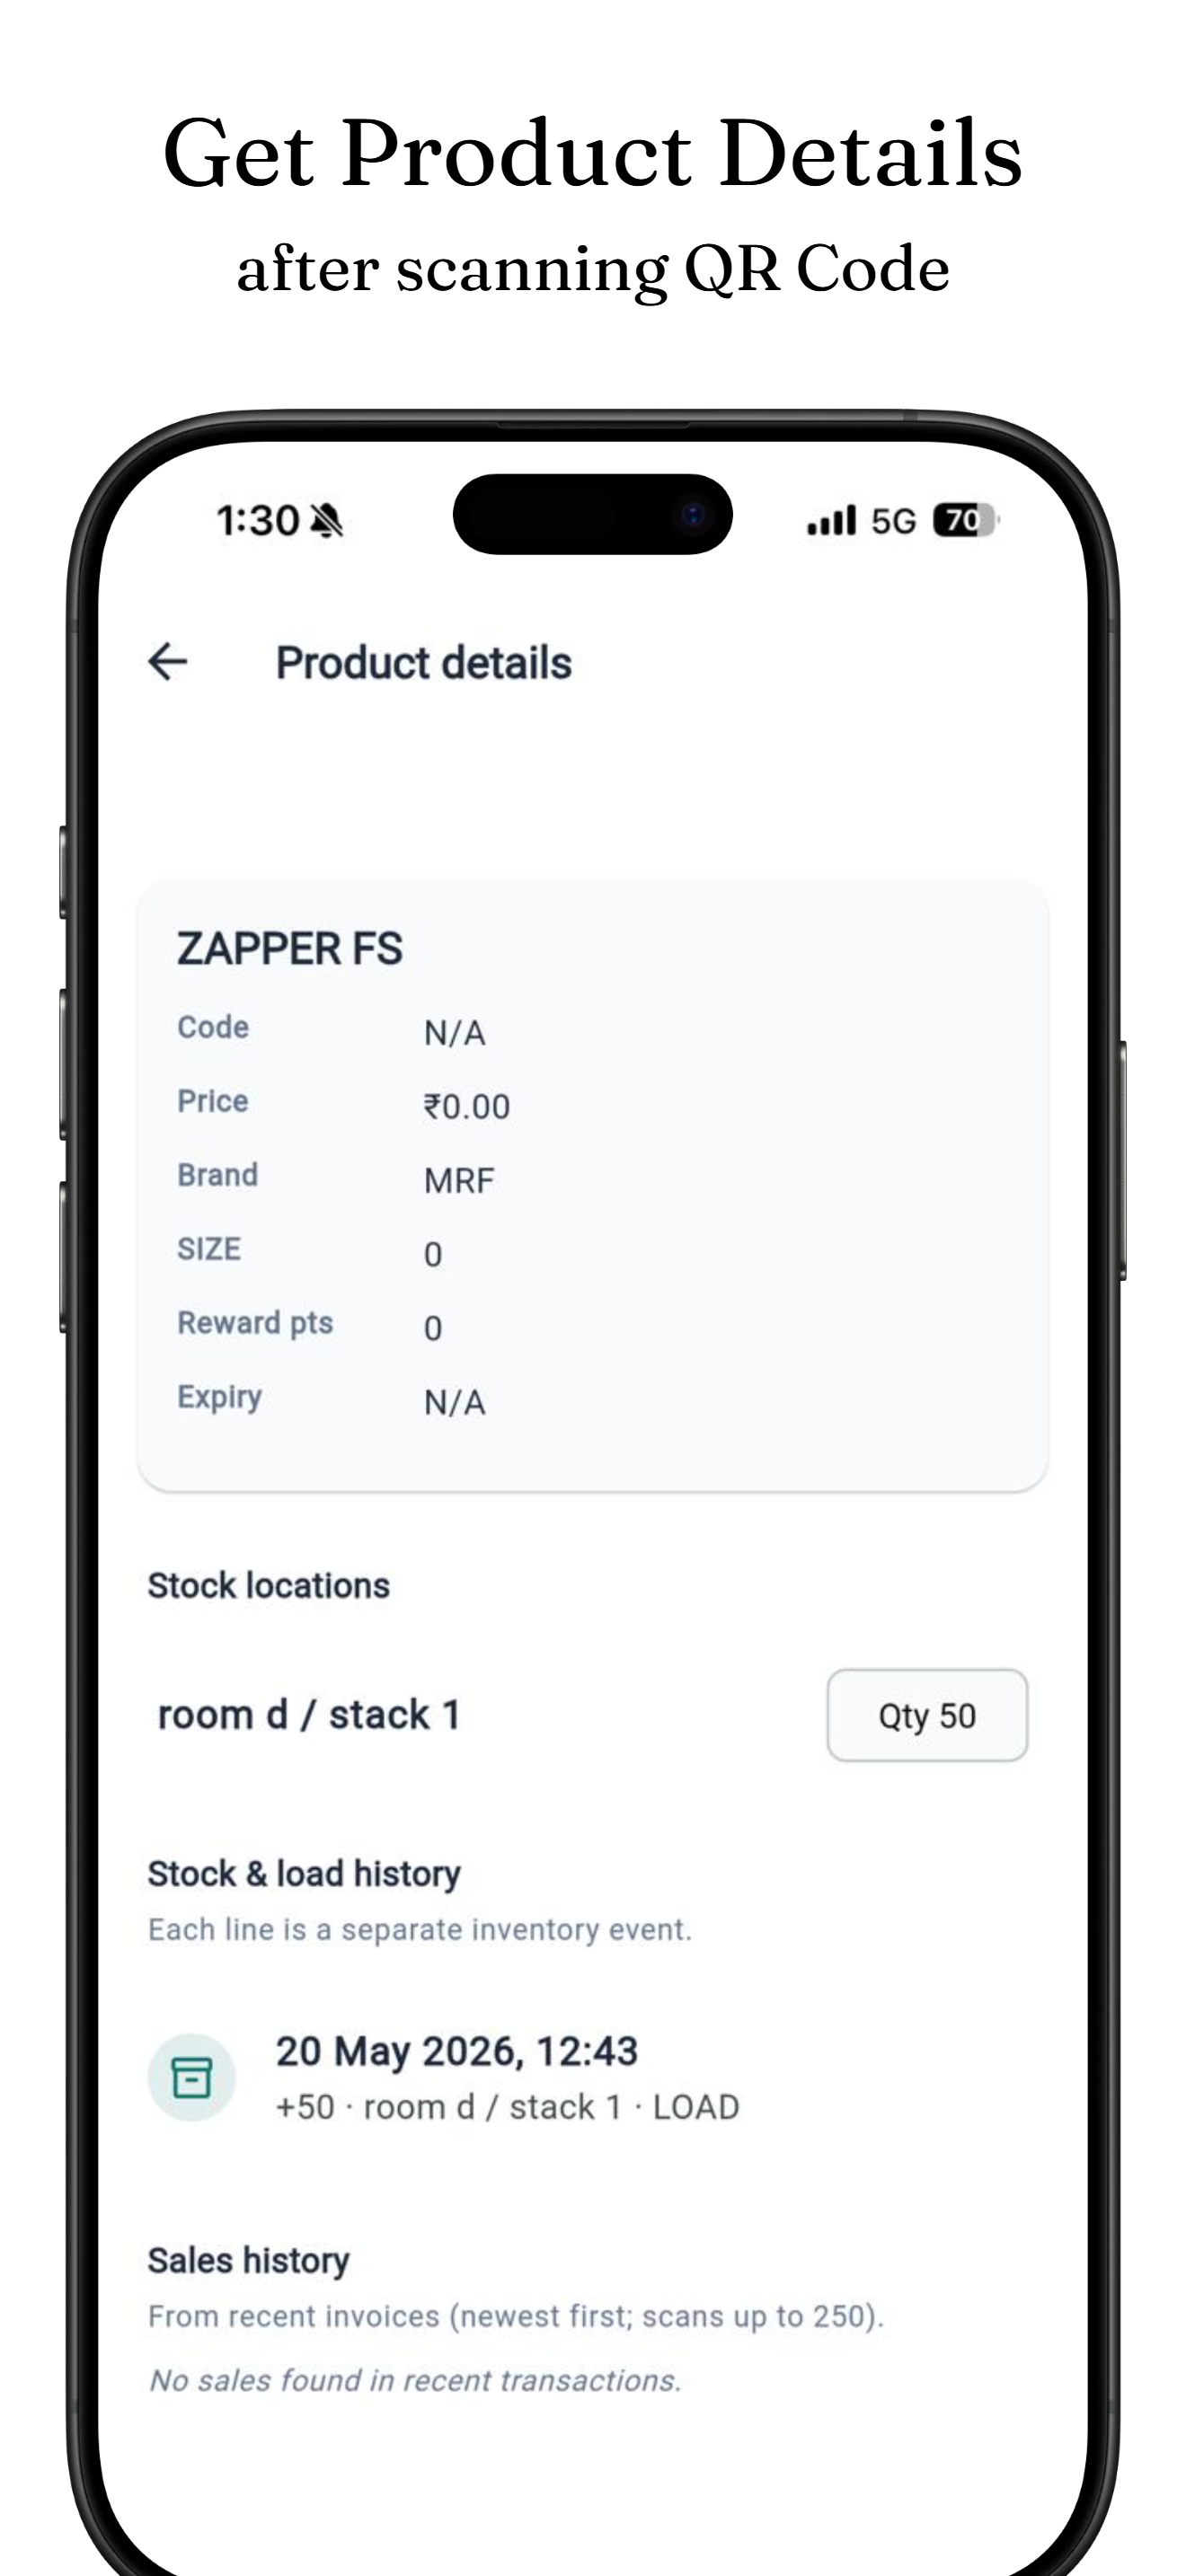
\includegraphics[width=\linewidth]{details_qr.png}
        \caption{Product Details using QR}
        \label{fig:details_qr}
    \end{minipage}
    \caption{Customer Management and QR-based Features}
    \label{fig:screens_set2}
\end{figure}

\begin{figure}[H]
    \centering
    \begin{minipage}{0.22\textwidth}
        \centering
        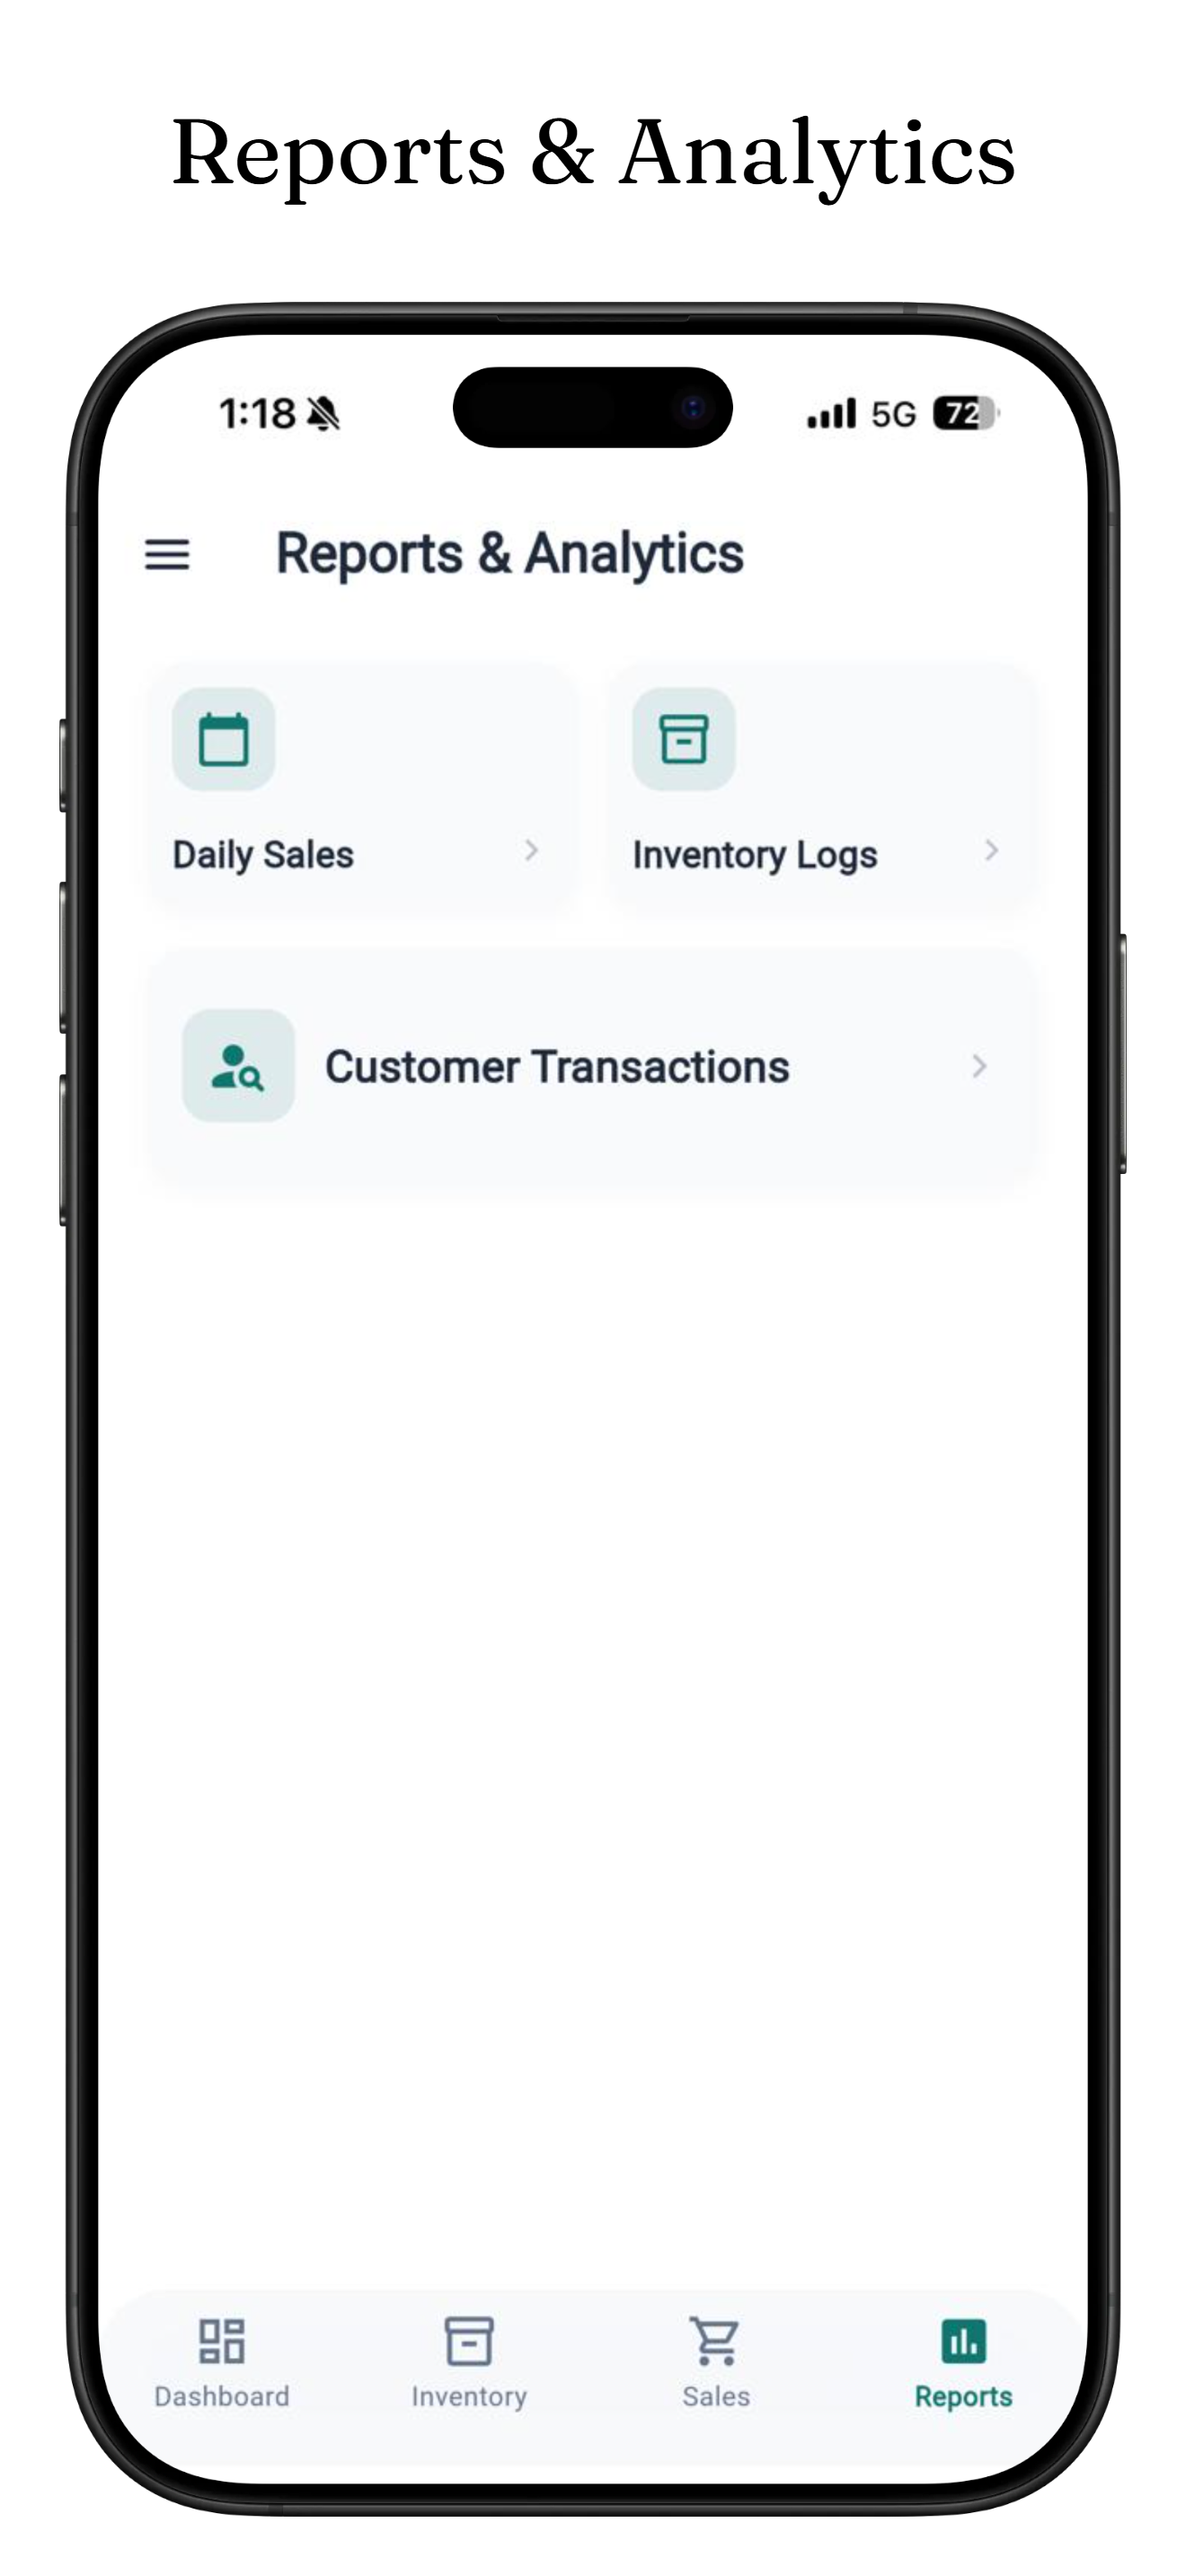
\includegraphics[width=\linewidth]{reports.png}
        \caption{Reports and Analytics}
        \label{fig:reports}
    \end{minipage}\hfill
    \begin{minipage}{0.22\textwidth}
        \centering
        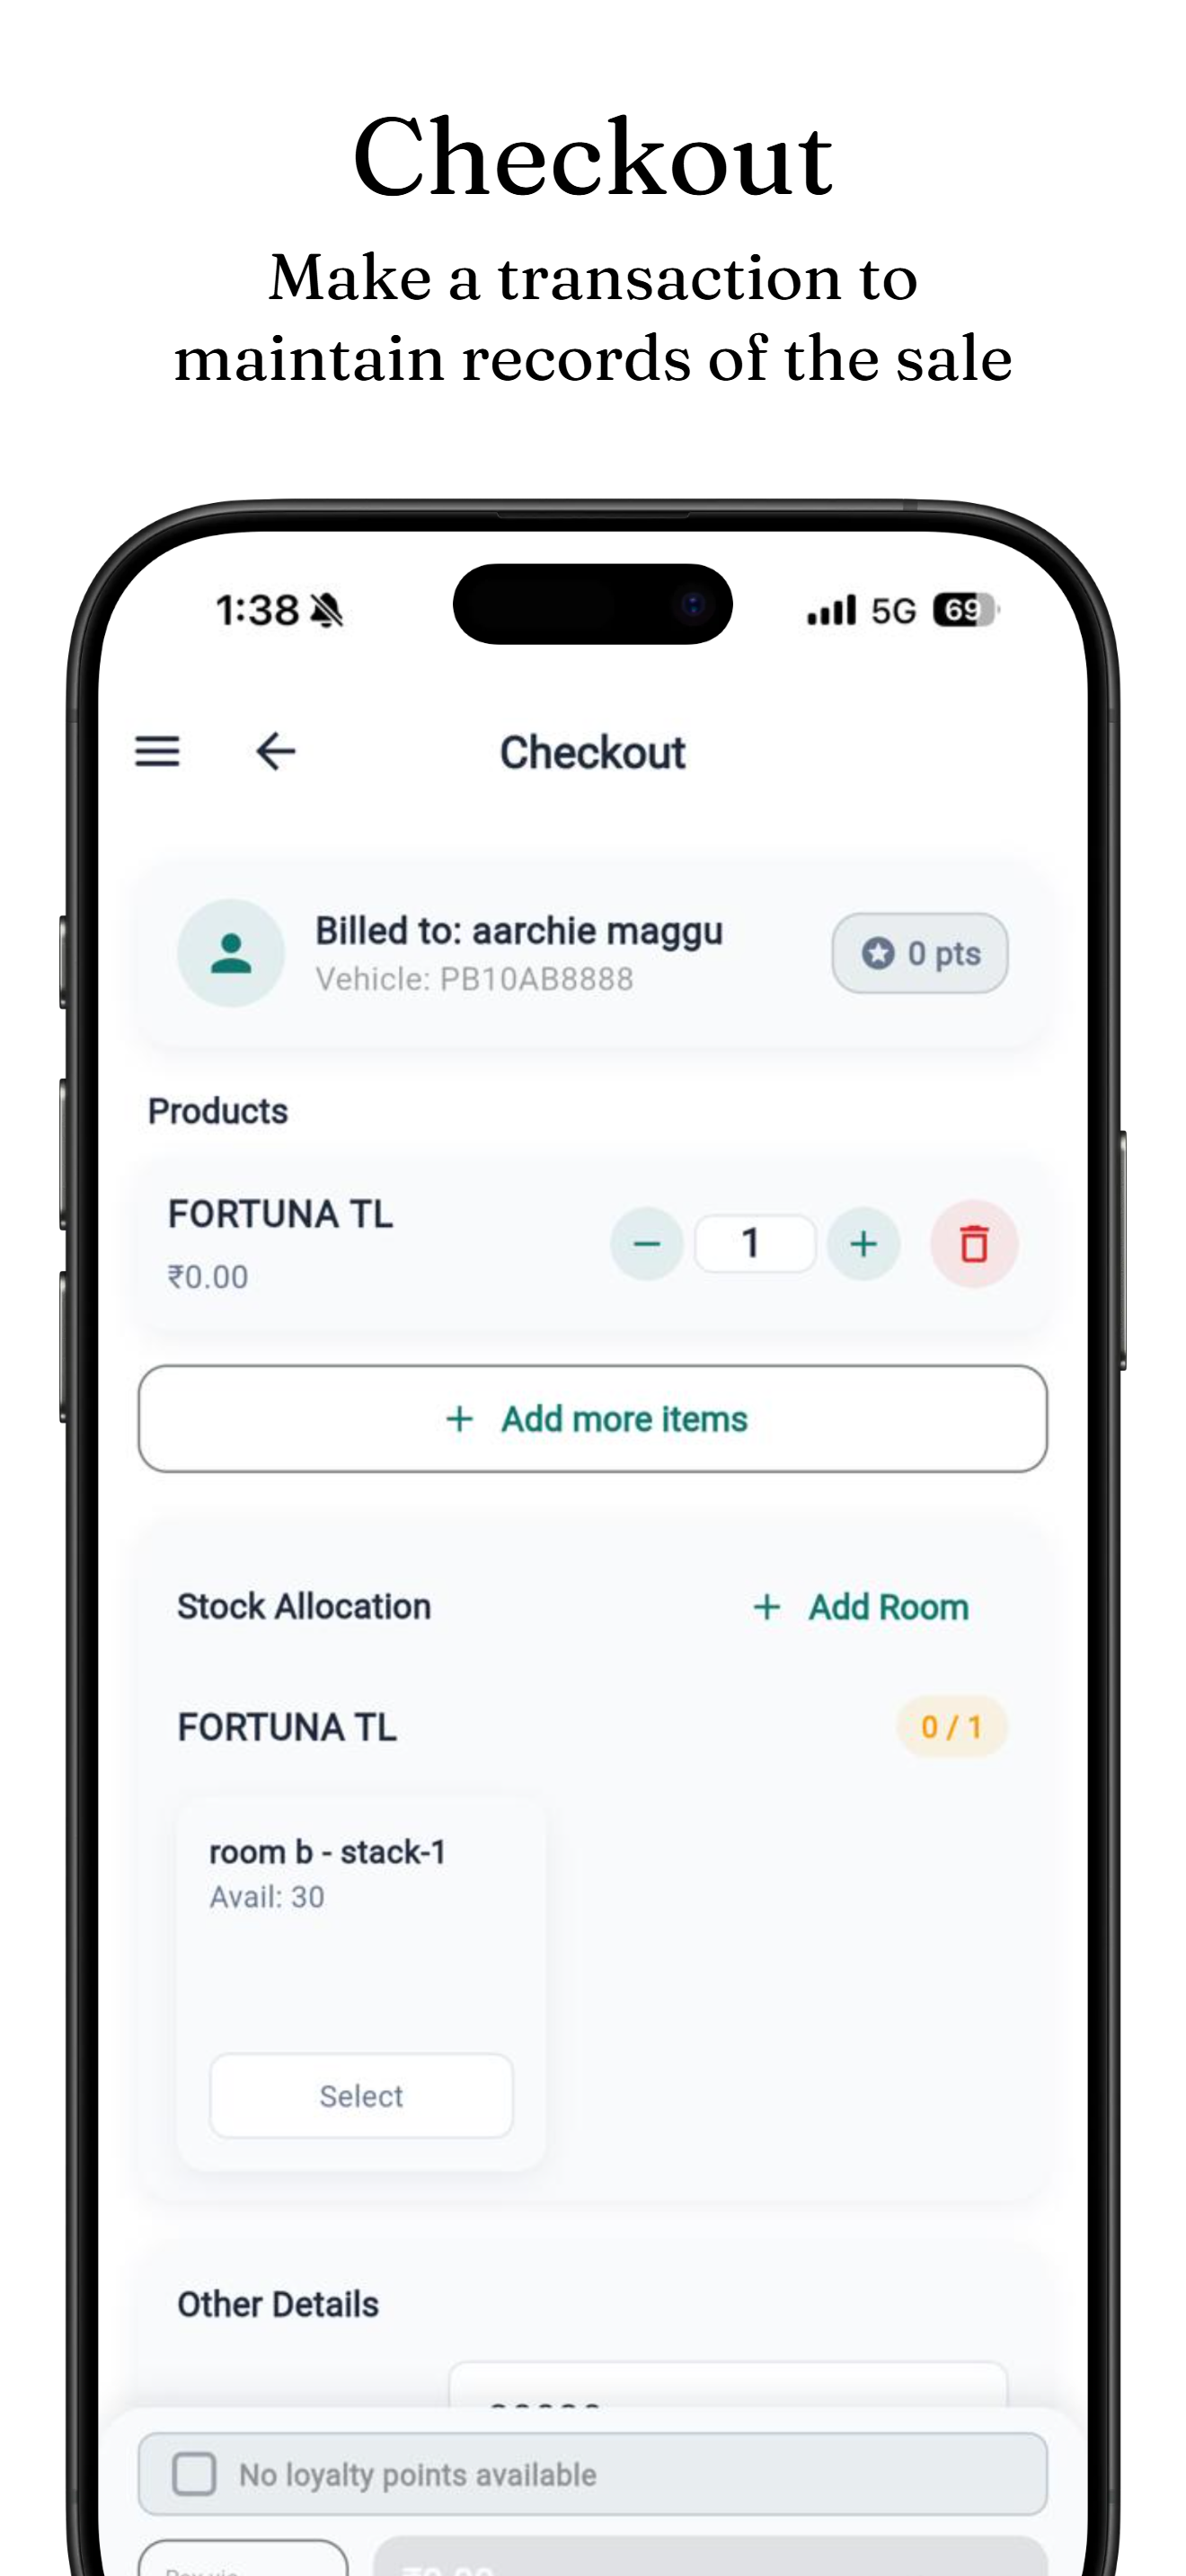
\includegraphics[width=\linewidth]{checkout.png}
        \caption{Checkout Page}
        \label{fig:checkout}
    \end{minipage}\hfill
    \begin{minipage}{0.22\textwidth}
        \centering
        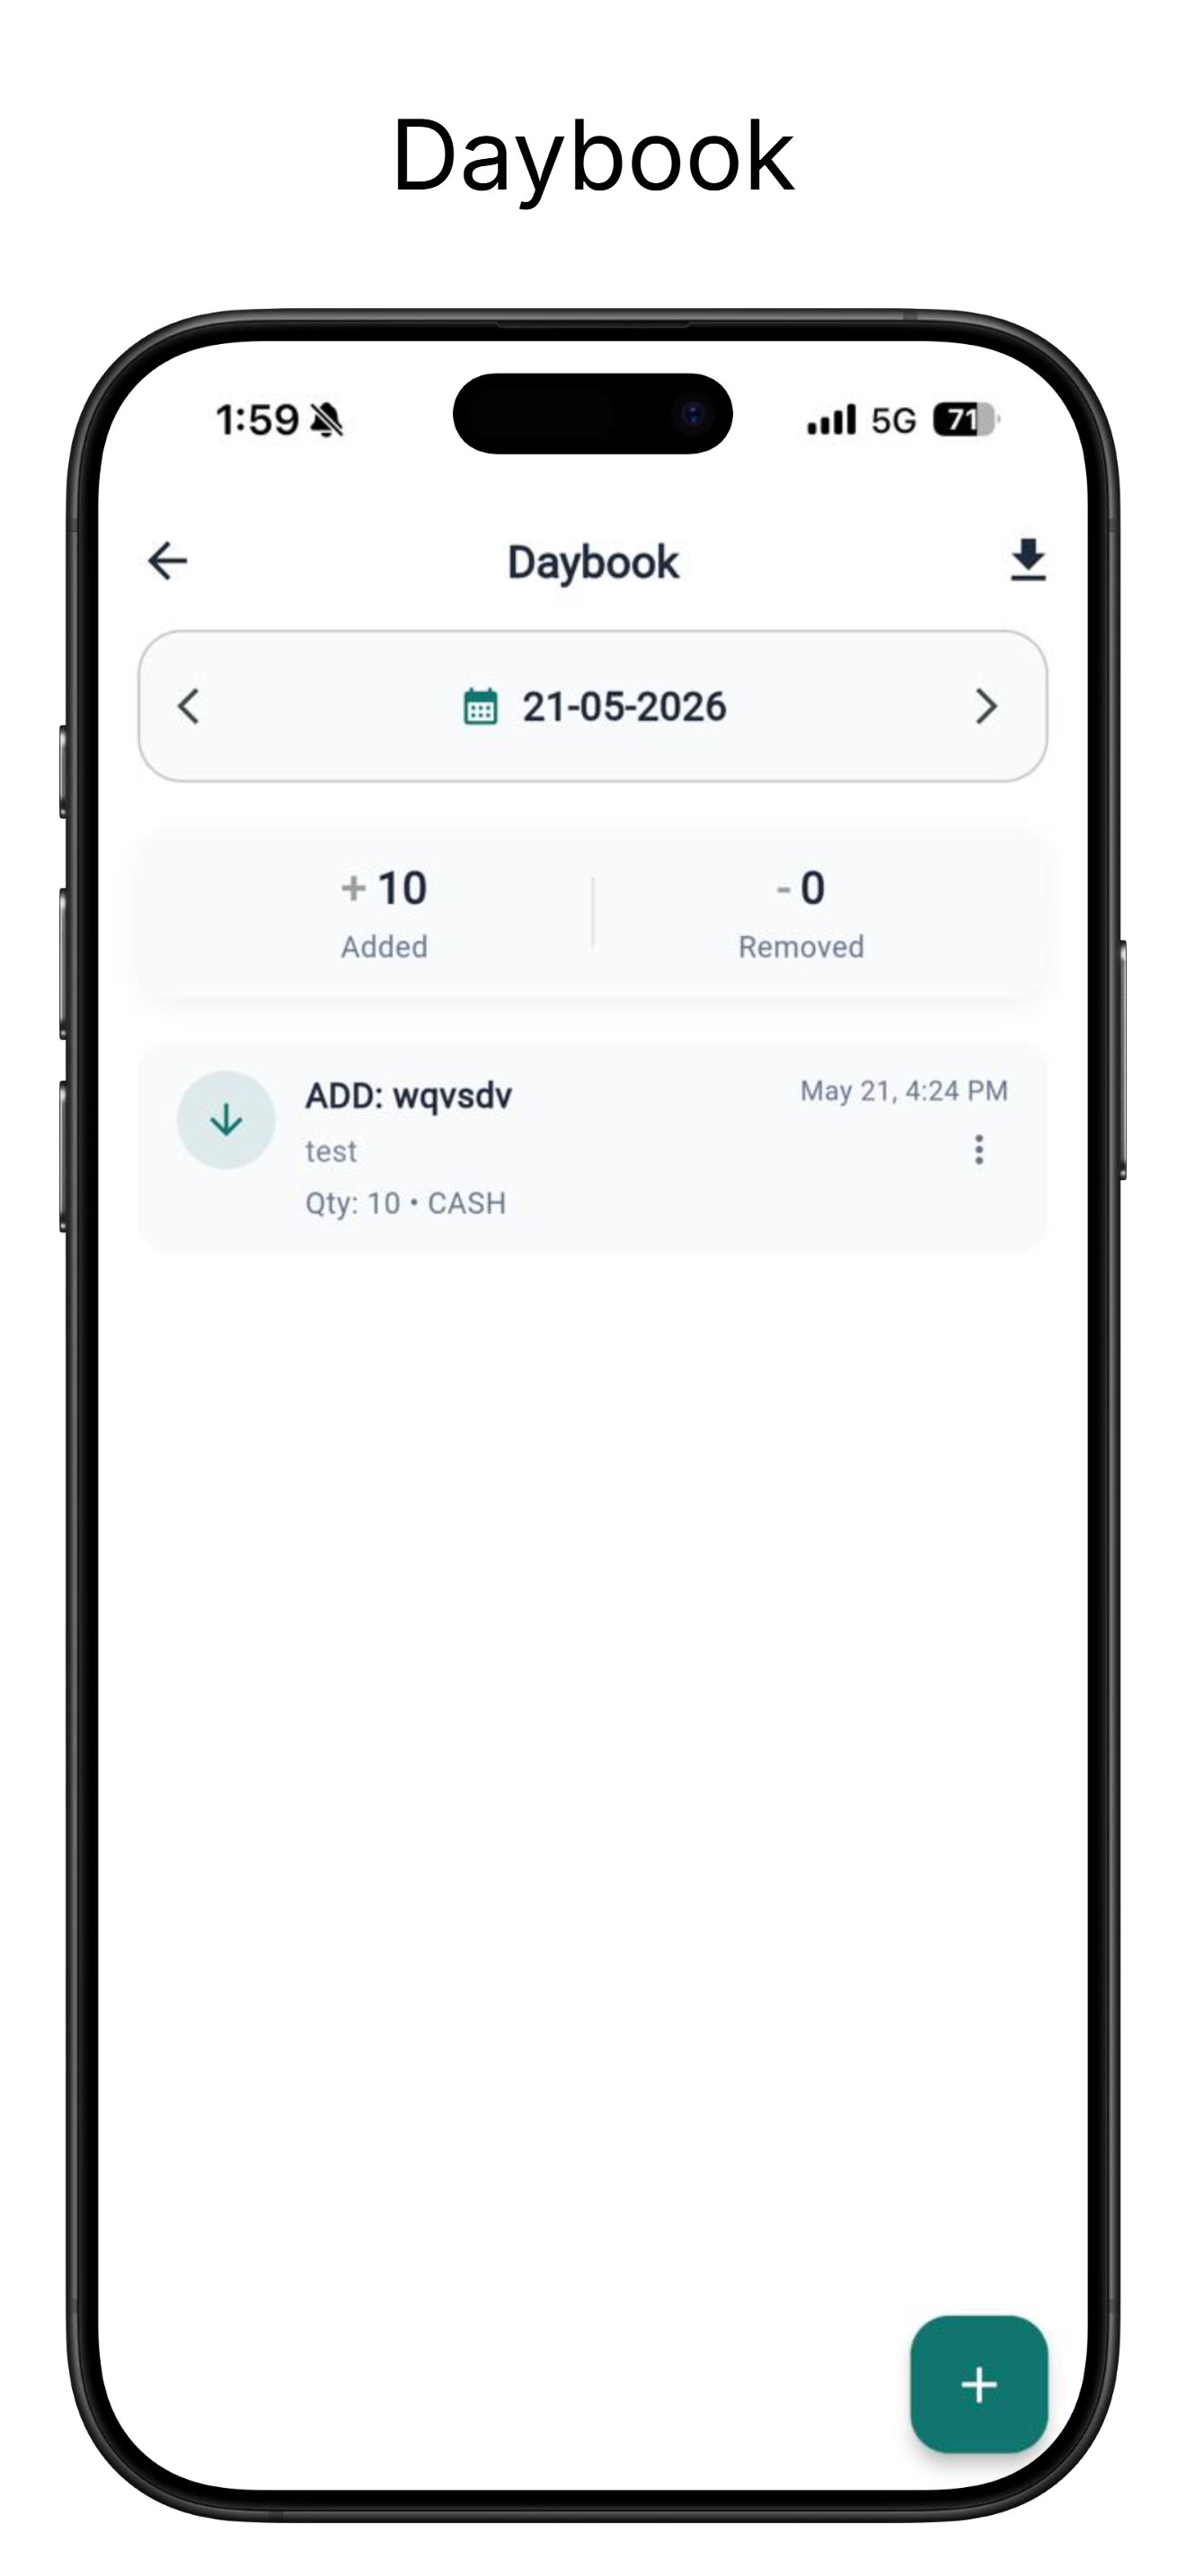
\includegraphics[width=\linewidth]{daybook.png}
        \caption{Daybook}
        \label{fig:daybook}
    \end{minipage}
    \caption{Reports, Checkout, and Daybook Screens}
    \label{fig:screens_set3}
\end{figure}

\begin{figure}[H]
    \centering
    \begin{minipage}{0.6\textwidth}
        \centering
        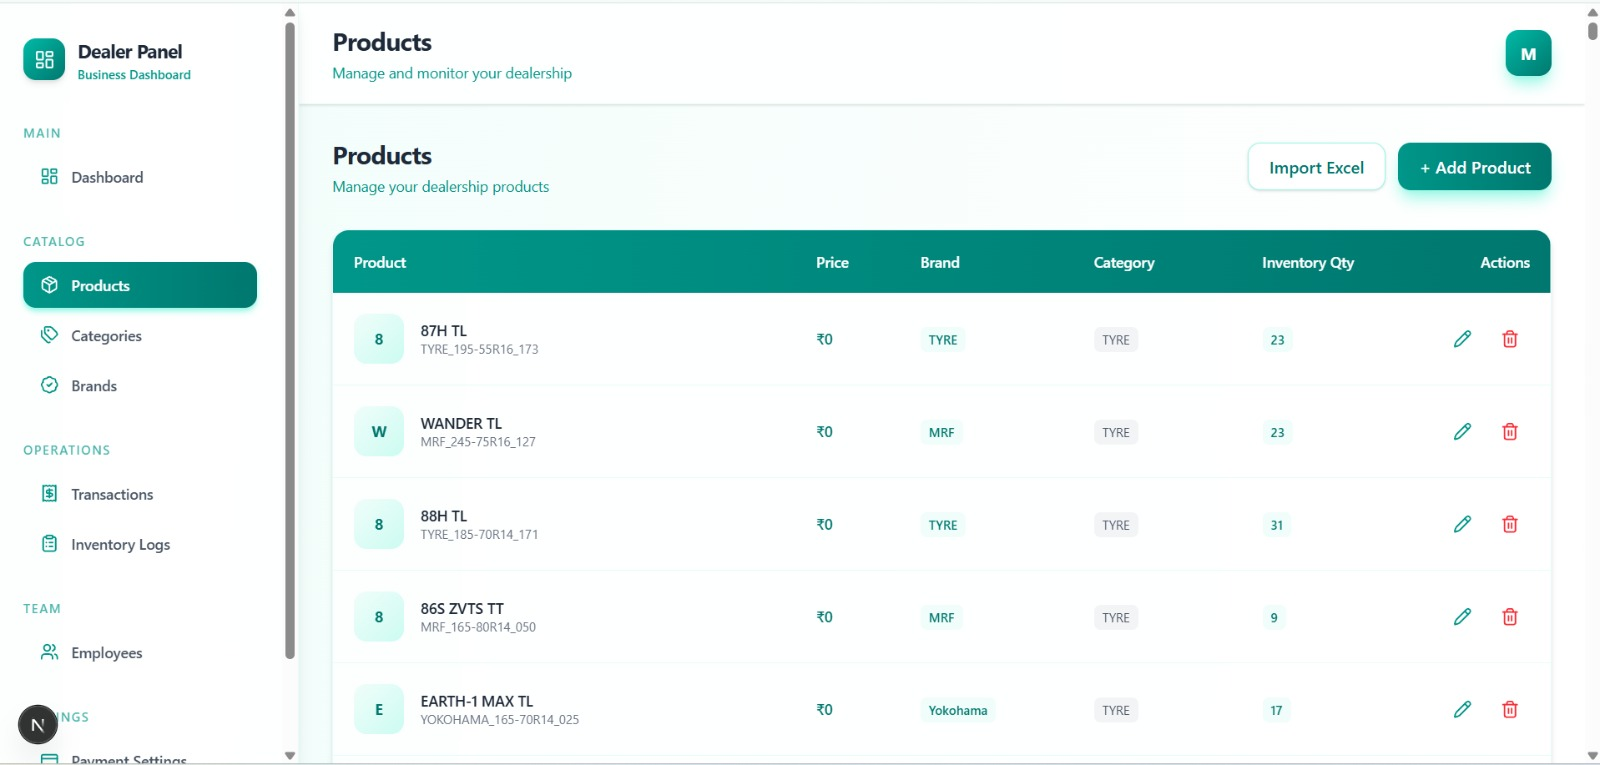
\includegraphics[width=\linewidth]{web_portal.jpeg}
        \caption{Web Portal — Worker Management}
        \label{fig:web_portal}
    \end{minipage}
    \caption{Web Portal Screen}
    \label{fig:screens_set4}
\end{figure}

\subsection*{6.4 Backend Representation}
\addcontentsline{toc}{subsection}{6.4 Backend Representation}

The backend of Trackit is built entirely on Firebase's managed cloud infrastructure. Cloud
Firestore serves as the primary real-time NoSQL database, organizing all business data into
structured collections as described in the database design chapter. Firebase Authentication
manages all user credentials and session handling, while Firebase Hosting supports backend
function deployment and the NextJS web portal is served through Vercel.

The following table summarizes the primary Firestore collections and the volume of data
operations observed during functional testing:

\renewcommand{\arraystretch}{1.4}
\begin{longtable}{|p{4cm}|p{4.5cm}|p{5cm}|}
\caption{Firestore Collections and Observed Data Operations} \label{tab:backend-ops} \\
\hline
\textbf{Collection} & \textbf{Primary Operations} & \textbf{Validation Outcome} \\
\hline
\endfirsthead
\multicolumn{3}{c}%
{{\bfseries \tablename\ \thetable{} -- continued from previous page}} \\
\hline
\textbf{Collection} & \textbf{Primary Operations} & \textbf{Validation Outcome} \\
\hline
\endhead
\hline \multicolumn{3}{|r|}{{Continued on next page}} \\ \hline
\endfoot
\hline
\endlastfoot
\texttt{dealers} & Read on login, write on registration & Role identified correctly on all test
logins \\
\hline
\texttt{workers} & Read on login, write on account creation, update on permission changes &
Permission changes reflected on next authenticated session \\
\hline
\texttt{customers} & Read for search, write on addition, update on edit & Search results
accurate for partial name and contact queries \\
\hline
\texttt{transactions} & Write on sale confirmation, read for history and daybook & All
transactions recorded with correct item, price, and customer references \\
\hline
\texttt{inventory} & Read for stock view, write/update on additions and adjustments & Real-time
stock updates reflected across devices within threshold \\
\hline
\texttt{inventory\_logs} & Write on every stock operation & All operations logged with correct
metadata and timestamps \\
\hline
\texttt{daybook} & Write on transaction confirmation, read for daily summary & Daily totals
computed and displayed correctly \\
\hline
\texttt{warranty\_links} & Read from transaction view, write by dealer & Warranty portals
accessible directly from customer transaction screen \\
\hline
\end{longtable}
\newpage
\begin{center}
    \section*{Chapter 7: Conclusion and Future Scope}
    \addcontentsline{toc}{section}{7. Conclusion and Future Scope}
\end{center}

\subsection*{7.1 Conclusion}
\addcontentsline{toc}{subsection}{7.1 Conclusion}

Trackit is a SaaS-based Inventory Management System developed to address the operational
challenges faced by tyre dealers in managing customer records, inventory, sales, and employee
activities through manual and semi-digital methods. The system provides a centralized,
cloud-based platform accessible through a Flutter-based cross-platform mobile application
and a NextJS-based web portal, both integrated with Firebase for real-time synchronization,
authentication, and secure data storage.\\[0.25cm]
The project successfully achieved all defined objectives. The Room-Stack Inventory Management
System provides a structured and efficient approach to organizing tyre stock according to
the physical layout of the dealer's warehouse. The permission-based employee access system
allows dealers to manage worker responsibilities with granular control, improving operational
security and workflow organization. The cart-based sales logging workflow, daybook management,
customer transaction history, and PDF export features collectively provide dealers with a
comprehensive digital solution that significantly reduces manual effort and minimizes the
risk of data errors.\\[0.25cm]
The system was validated through iterative testing across all modules, confirming functional
correctness, real-time synchronization reliability, cross-platform compatibility, and
role-based access enforcement. The use of Firebase's serverless, auto-scaling infrastructure
ensures that the system remains cost-effective and operationally sustainable as the dealer's
customer base and inventory volume grow over time.\\[0.25cm]
Overall, Trackit demonstrates that a well-designed, cloud-based SaaS platform can effectively
replace traditional manual record-keeping practices in small and medium-scale retail businesses,
providing measurable improvements in efficiency, data accuracy, and business organization.


\subsection*{7.2 Future Scope}
\addcontentsline{toc}{subsection}{7.2 Future Scope}

While Trackit fulfills its current set of requirements comprehensively, several enhancements
and extensions have been identified that can further improve the system's capabilities and
broaden its applicability in the future:

\begin{enumerate}

    \item \textbf{Automated Low-Stock Alerts and Reorder Notifications:} The system can be
    extended to automatically detect when inventory levels for a particular tyre brand or
    size fall below a predefined threshold and notify the dealer through in-app alerts or
    push notifications, enabling proactive stock replenishment.

    \item \textbf{Multi-Shop Support for Dealer Chains:} Future versions of Trackit can
    introduce support for dealers who operate multiple shop locations, allowing centralized
    management of inventory, sales, and employees across all branches from a single dealer
    account.

    \item \textbf{Supplier and Purchase Order Management:} A dedicated supplier management
    module can be added to allow dealers to maintain supplier records, raise digital purchase
    orders, and track incoming inventory against outstanding orders, further streamlining
    the supply chain workflow.

    \item \textbf{Customer Loyalty and Service Reminder System:} The platform can be enhanced
    to send automated service reminders to customers based on vehicle mileage or the elapsed
    time since their last tyre purchase, improving customer retention and after-sales
    engagement.

    \item \textbf{Advanced Analytics and Business Intelligence Dashboard:} More sophisticated
    reporting capabilities, including trend analysis, seasonal demand forecasting, top-selling
    product identification, and profitability reports, can be integrated to provide dealers
    with deeper insights for informed business decision-making.

    \item \textbf{Offline Mode with Local Data Caching:} The mobile application can be
    enhanced with offline support using local data caching strategies, allowing dealers and
    workers to continue performing essential operations such as sales logging and customer
    lookup during periods of limited or no internet connectivity, with automatic
    synchronization upon reconnection.

    \item \textbf{Barcode and QR Code Integration:} Integration of barcode or QR code scanning
    functionality can accelerate inventory management operations by allowing workers to scan
    tyre packaging directly to add or locate stock, reducing manual data entry time and the
    risk of input errors.

    \item \textbf{Expansion to Other Automotive Retail Segments:} The core architecture of
    Trackit, particularly the Room-Stack inventory model and permission-based access system,
    can be adapted for use by dealers in adjacent automotive retail segments such as batteries,
    lubricants, and spare parts, expanding the platform's commercial applicability.

    \item \textbf{Third-Party Accounting Software Integration:} Future development can include
    integration with widely used accounting and GST billing platforms, allowing transaction
    data recorded in Trackit to be automatically exported to accounting systems, reducing
    duplication of effort in financial reporting.

\end{enumerate}

\newpage
\begin{center}
    \LARGE \textbf{References}
\end{center}
\addcontentsline{toc}{section}{8. References}
\vspace{-2.6 em}
\renewcommand{\refname}{}
\bibliographystyle{plainnat}
\begin{thebibliography}{99}

\bibitem{firebase}
Google. (2026). Firebase Documentation [Online]. Available: https://firebase.google.com/docs

\bibitem{flutter}
Flutter Team. (2026). Flutter Documentation [Online]. Available: https://docs.flutter.dev

\bibitem{nextjs}
Next.js Team. (2026). Next.js Documentation [Online]. Available: https://nextjs.org/docs

\bibitem{firestore}
Google Cloud. (2026). Cloud Firestore Documentation [Online]. Available: https://firebase.google.com/docs/firestore

\bibitem{inventory}
Oracle Corporation. (2026). Inventory Management Systems Overview [Online]. Available: https://www.oracle.com/scm/inventory-management/

\bibitem{saas}
Microsoft Azure. (2026). What is Software as a Service (SaaS)? [Online]. Available: https://azure.microsoft.com/en-us/resources/cloud-computing-dictionary/what-is-saas/

\bibitem{vercel}
Vercel. (2026). Vercel Platform Documentation [Online]. Available: https://vercel.com/docs

\bibitem{github}
GitHub. (2026). GitHub Documentation [Online]. Available: https://docs.github.com/

\bibitem{flchart}
imaNNeo. (2026). fl\_chart Package [Online]. Available: https://pub.dev/packages/fl\_chart

\bibitem{pdfpkg}
DavidPH. (2026). pdf Package [Online]. Available: https://pub.dev/packages/pdf

\bibitem{auribises}
Auribises Technologies. (2026). Auribises Technologies Official Website [Online]. Available: https://auribises.com

\end{thebibliography}


\end{document}
